\chapter{Quantum Fourier Transform}

One of the most remarkable features of quantum computers is their ability to perform certain computational tasks exponentially faster than classical computers. A prominent example of this is prime factorization. Shor’s algorithm, proposed in the 1990s, demonstrated that an $n$-bit integer can be factored in $O(n^2 \log n \log \log n)$ operations on a quantum computer. This is an exponential improvement over the best-known classical algorithm at the time, the number field sieve, which required $O\left(\exp\left(\Theta(n^{1/2} \log^{2/3} n)\right)\right)$ operations. On a classical machine, factoring large integers quickly becomes infeasible, as the computational cost grows exponentially with the size (Number of bits - $n$) of the number. In contrast, quantum computers can achieve this in polynomial time, making Shor's result a landmark demonstration of quantum computational power.

This naturally raises an exciting question: What other problems can quantum computers solve efficiently that are intractable for classical ones?

A key ingredient in Shor's algorithm is the \textbf{Quantum Fourier Transform (QFT)}. This transform lies at the heart of the quantum phase estimation (QPE) algorithm, which is fundamental to finding the eigenvalues of unitary operators under certain conditions— a topic we will explore in the next chapter. The QPE enabled by QFT also plays a central role in solving the order-finding problem and the discrete logarithm problem, both of which were previously considered hard for classical computation. These problems and their quantum solutions can be understood as instances of a broader framework known as the \textit{Hidden Subgroup Problem}.

Moreover, quantum phase estimation is used to count the number of solutions to certain search problems, revealing how foundational QFT is to quantum speedups. In many of these algorithms, the exponential advantage stems from the efficiency of the Quantum Fourier Transform itself.

The QFT is the quantum analog of the classical Discrete Fourier Transform (DFT). DFT spans a wide variety of applications in numerous fields from Signal processing, image and video processing, telecommunications, control systems to geophysics and medical imagining. In many areas of science and engineering, whenever a signal exhibits periodic behavior and one wishes to extract its frequency components, the Fourier transform is the tool of choice. There are several variants of the Fourier transform — continuous, discrete, Boolean, etc. In essence, Fourier analysis provides a mathematical lens for examining the internal frequencies of a function.

Finally, the QFT can be seen as a generalization of the Hadamard transform. Both produce superpositions, but the QFT introduces complex phases — specifically, powers of the primitive roots of unity, denoted by $\omega$. These phases are what give QFT its distinctive interference patterns and computational power.

In the sections that follow, we begin by establishing the mathematical foundations necessary for understanding the Fourier transform, starting with the concept of roots of unity, which play a central role in the Discrete Fourier Transform (DFT). We then explore various approaches to computing the DFT, beginning with the naive method and progressing to the more efficient Fast Fourier Transform (FFT) algorithm. Building on this, we introduce the Quantum Fourier Transform (QFT), examining its definition, key properties, and several illustrative examples and applications. Both intuitive and rigorous mathematical approaches to efficiently implementing the QFT are discussed in detail along with the compelxity analysis. We also delve into the concept of the Approximate Quantum Fourier Transform (AQFT) and demonstrate the concept of how the Fourier transform can be used to perform operations such as modular addition. Special attention is given to scenarios where measurements occur at the end of quantum circuits, and we analyze how this can lead to simplifications and reductions in computational complexity. Finally, we conclude the chapter with a complete implementation of the Quantum Fourier Transform using Qiskit.

\section{Mathematical Foundations}
\subsection{Roots of Unity}

\begin{definition}[Roots of Unity]
The $N$th roots of unity are the complex solutions to the equation:
\begin{equation}
    z^N = 1.
    \label{eq:root_unity_equation}
\end{equation}
Recall the Fundamental Theorem of Algebra, 
\begin{lemma}[Fundamental Theorem of Algebra]
    Every non-zero, single-variable, degree $n$ polynomial with complex coefficients has, counted with multiplicity, exactly $n$ complex roots.
\end{lemma}
By the Fundamental Theorem of Algebra, this equation has exactly $N$ distinct complex solutions in the field $\mathbb{C}$. For example:
\begin{itemize}
    \item If $N = 2$, the solutions are $z = 1$ and $z = -1$.
    \item If $N = 4$, the solutions are $z = 1, i, -1, -i$.
\end{itemize}
These roots can be expressed as powers of a primitive $N$th root of unity:
\begin{equation}
    \omega_N = e^{2\pi\iota / N},
\end{equation}
so that the $k$th root is:
\begin{equation}
    \omega_N^k = e^{2\pi\iota k / N}, \quad \text{for } k = 0, 1, \dots, N-1.
    \label{eq:omega_powers}
\end{equation}
\end{definition}

\noindent
Each root $\omega_N^k$ lies on the complex unit circle in $\mathbb{C}$, since:
\[
|\omega_N^k| = \left| e^{2\pi\iota k / N} \right| = 1.
\]
These roots are equally spaced around the circle, and each makes an angle:
\[
\phi_k = \frac{2\pi k}{N}
\]
with the positive real axis. Squaring $\omega_N$ doubles the angle, and in general, raising it to the $j$th power multiplies the angle by $j$, i.e., $\omega_N^j$ has argument $\frac{2\pi j}{N}$ and remains an $N$th root of unity.

\begin{figure}[H]
    \centering
    \begin{tikzpicture}[scale=2]
        \draw[->] (-1.2,0) -- (1.5,0) node[right] {$\Re$};
        \draw[->] (0,-1.2) -- (0,1.5) node[above] {$\Im$};
        \draw (0,0) circle(1);
        \foreach \k in {0,...,4} {
            \filldraw[black] ({cos(72*\k)}, {sin(72*\k)}) circle (1pt);
            \node at ({1.25*cos(72*\k)}, {1.25*sin(72*\k)}) {$\omega^{{\k}}$};
        }
    \end{tikzpicture}
    \caption{The fifth roots of unity ($N = 5$) on the complex plane}
    \label{fig:rootsofunity}
\end{figure}

\subsubsection*{Properties of Roots of Unity}

\begin{itemize}
    \item \textbf{Periodicity:} The roots are periodic modulo $N$, i.e.,
    \begin{equation}
        \omega_N^k = \omega_N^{k \bmod N}.
        \label{eq:periodicity}
    \end{equation}
    \begin{example}
        For $N = 4$, the roots are:
        \[
        \omega_4^0 = e^{2\pi\iota \cdot 0 / 4} = 1, \quad \omega_4^1 = i, \quad \omega_4^2 = -1, \quad \omega_4^3 = -i.
        \]
        This confirms that $k \bmod 4$ wraps around the unit circle.
    \end{example}
    
    \item \textbf{Sum of All Roots:} The sum of all $N$th roots of unity is zero:
    \begin{equation}
        \sum_{k=0}^{N-1} \omega_N^k = 0.
        \label{eq:roots_sum}
    \end{equation}
    
    \item \textbf{Geometric Sum Property:} More generally, for all $k \in \{1,2,\dots,N-1\}$:
    \begin{equation}
        \sum_{j=0}^{N-1} \omega_N^{kj} = 0,
        \label{eq:sum_powers_of_omega}
    \end{equation}
    since $\omega_N^k$ is a nontrivial $N$th root of unity and the geometric sum evaluates to zero when $\omega_N^k \neq 1$.
    
    \item \textbf{Special Case for $k = 0$:}
    \begin{equation}
        \sum_{j=0}^{N-1} \omega_N^{0 \cdot j} = \sum_{j=0}^{N-1} 1 = N.
        \label{eq:trivial_sum}
    \end{equation}
\end{itemize}

\begin{remark}
The equal spacing, symmetry, and periodicity of the roots of unity make them fundamental to the structure of the Discrete Fourier Transform (DFT), which uses these roots in its matrix representation (see Equation~\eqref{eq:dft_matrix}).
\end{remark}

\subsection{The Discrete Fourier Transform}
One of the most powerful strategies in mathematics and computer science is to transform a difficult problem into another form for which an efficient solution is known. Among such transformations, the \textit{Fourier transform} stands out due to its widespread utility across diverse fields. In particular, the \textit{Discrete Fourier Transform (DFT)} appears frequently in signal processing, systems analysis, and quantum computation. In this chapter, we will focus on the Quantum Fourier Transform (QFT), which is essentially the quantum analogue of the classical Discrete Fourier Transform (DFT). The QFT will be the central theme throughout the rest of the chapter and will form the backbone of many quantum algorithms we study.

\subsubsection{Definition of the DFT}
\begin{definition}[Discrete Fourier Transform (DFT)]
    The \textit{Discrete Fourier transform (DFT)} takes as input a vector of complex numbers, \( \vec{x} = \begin{bmatrix}
        x_0 & \ldots x_{N-1}        
    \end{bmatrix}^\top\) where the length $N$ of the vectors is a fixed parameter. It outputs the transformed data, a vector of complex numbers \(\vec{y}= \begin{bmatrix} y_0 & \ldots & y_{N-1}\end{bmatrix}^\top\), defined by
\begin{equation}
y_k = \frac{1}{\sqrt{N}} \sum_{j=0}^{N-1} x_je^{2\pi\iota jk/N} \quad \text{for } k=0,\ldots,N-1
\label{eq:dft}
\end{equation}
\end{definition}
\begin{definition}[Discrete Fourier Transform Matrix]

Let $N$ be a positive integer and let \(\omega_N = e^{2\pi\iota / N}\) be the primitive $N$th root of unity. The \(N \times N\) Discrete Fourier Transform matrix $DFT_N$ is defined as:
\begin{equation}
    (DFT_N)_{jk} = \frac{1}{\sqrt{N}} \omega_N^{jk}, \quad \text{for } 0 \leq j,k < N.
    \label{eq:dft_matrix_entry}
\end{equation}
Explicitly, the DFT matrix is:
\begin{equation}
    DFT_N = \frac{1}{\sqrt{N}}\begin{pmatrix}
        1 & 1 & 1 & \cdots & 1 \\
        1 & \omega_N & \omega_N^2 & \cdots & \omega_N^{N-1} \\
        1 & \omega_N^2 & \omega_N^4 & \cdots & \omega_N^{2(N-1)} \\
        \vdots & \vdots & \vdots & \ddots & \vdots \\
        1 & \omega_N^{N-1} & \omega_N^{2(N-1)} & \cdots & \omega_N^{(N-1)^2}
    \end{pmatrix}.
    \label{eq:dft_matrix}
\end{equation}
\end{definition}
In general, the DFT can be thought of as follows:
\[
\dfrac{1}{\sqrt{N}}\begin{bmatrix} 1 & 1 & 1 & \ldots & 1 \\ 1 & \omega_N & \omega_N^2 & \ldots & \omega_N^{N-1} \\ 1 & \omega_N^2 & \omega_N^4 & \ldots & \omega_N^{2(N-1)} \\ \vdots & \vdots & \vdots & \ddots & \vdots \\ 1 & \omega_N^{N-1} & \omega_N^{2(N-1)} & \ldots & \omega_N^{(N-1)(N-1)} \end{bmatrix}\begin{bmatrix} x_0 \\ x_1 \\ \vdots \\ x_{N-1} \end{bmatrix} = \begin{bmatrix} y_0 \\ y_1 \\ \vdots \\ y_{N-1} \end{bmatrix} = \sum_{k=0}^{N-1} \sum_{j=0}^{N-1} x_j e^{2\pi\iota jk/N}\ket{k}
\]
where $\omega_N=e^{2\pi\iota /N}$.
\subsection{Computing the Discrete Fourier Transform}
\subsubsection{Naïve Method}

The most straightforward approach to computing the Discrete Fourier Transform (DFT) of a vector $\vec{x} \in \mathbb{C}^N$ is through direct matrix-vector multiplication:

\begin{equation}
    \vec{y} = DFT_N \vec{x},
\end{equation}

where $DFT_N \in \mathbb{C}^{N \times N}$ is the DFT matrix. This method, often referred to as the \textbf{naïve} method, involves computing each entry of $\vec{y}$ as a linear combination of the entries of $\vec{x}$ using the complex exponentials $e^{2\pi\iota ij/N}$ in the DFT matrix. Each output component $y_k$ requires $O(N)$ operations—specifically, $2N$ additions and $4N$ multiplications (assuming complex arithmetic). Therefore, computing all $N$ components of $\vec{y}$ requires a total of $O(N^2)$ operations.

While simple and intuitive, this approach becomes computationally inefficient for large $N$, motivating the development of faster algorithms such as the Fast Fourier Transform (FFT), which is discussed in the next section.

\subsubsection{Fast Fourier Transform (FFT)}

A significantly more efficient method for computing $\vec{y} = DFT_N \vec{x}$ is the \textit{Fast Fourier Transform} (FFT), introduced by Cooley and Tukey in 1965~\cite{cooley1965algorithm}. This algorithm reduces the computational complexity from $O(N^2)$ to $O(N \log N)$, which constitutes a tremendous improvement when $N$ is large. This improvement is a key reason why Fourier transforms are so widely used in practice. The FFT has had a profound impact on signal processing and digital computation—it underlies virtually all modern electronic systems. Without FFT, many capabilities of current technology would be infeasible or prohibitively slow.

The FFT algorithm assumes that $N = 2^n$ for some integer $n$, a condition that is usually easy to satisfy in practice by zero-padding input vectors. Moreover, variants of FFT exist that can handle non-power-of-two values of $N$. The key insight of the FFT is to exploit the symmetry and periodicity of the complex roots of unity in the DFT matrix to recursively reduce the computation. We rewrite the DFT of size $N$ in terms of two DFTs of size $N/2$, applied to the even- and odd-indexed elements of $\vec{x}$:

\begin{align}
    y_j &= \frac{1}{\sqrt{N}} \sum_{k=0}^{N-1} \omega_N^{jk} x_k \nonumber \\
        &= \frac{1}{\sqrt{N}} \left( \sum_{\substack{k=0 \\ k \text{ even}}}^{N-1} \omega_N^{jk} x_k + \sum_{\substack{k=0 \\ k \text{ odd}}}^{N-1} \omega_N^{jk} x_k \right) \nonumber \\
        &= \frac{1}{\sqrt{2}} \left( \frac{1}{\sqrt{N/2}} \sum_{k'=0}^{N/2 - 1} \omega_{N/2}^{j k'} x_{2k'} + \omega_N^j \cdot \frac{1}{\sqrt{N/2}} \sum_{k'=0}^{N/2 - 1} \omega_{N/2}^{j k'} x_{2k'+1} \right). \label{eq:fft-recursion}
\end{align}

Here, we have grouped the even and odd indexed terms, using the fact that $\omega_N^{2jk'} = \omega_{N/2}^{jk'}$ and factoring out the corresponding phase. This gives rise to a recursive procedure: compute the DFT of the even-indexed entries of $\vec{x}$ to obtain $\vec{y}_{\text{even}}$, and the DFT of the odd-indexed entries to obtain $\vec{y}_{\text{odd}}$. Then, the output entries are reconstructed as:

\begin{equation}
    y_j = \frac{1}{\sqrt{2}} \left( (\vec{y}_{\text{even}})_j + \omega_N^j (\vec{y}_{\text{odd}})_j \right), \quad \text{for } 0 \leq j < N.
\end{equation}

This formula appears to be ill-defined beyond $j \geq N/2$, as $\vec{y}_{\text{even}}$ and $\vec{y}_{\text{odd}}$ have only $N/2$ components each. However, we can extend them by periodicity:
\[
    (\vec{y}_{\text{even}})_{j + N/2} := (\vec{y}_{\text{even}})_j, \quad
    (\vec{y}_{\text{odd}})_{j + N/2} := (\vec{y}_{\text{odd}})_j.
\]
The time complexity $T(N)$ of this recursive algorithm satisfies the recurrence:
\[
T(N) = 2T(N/2) + O(N),
\]
with $T(2)=1$, which solves to $T(N) = O(N \log N)$. 

\textbf{(Cooley-Turkey Algorithm)}For each $x_k$ we can separate the sum into odd and even indices, then we require $2^n$ operations assuming the two separate sums are known. this can be done recursively, splitting each sum into $2$ pieces. This leads to the number of operations to be $\Theta(2^n \log_22^n) = \Theta(n2^n)$.

    A radix-2 decimation-in-time (DIT) FFT is the simplest and most common form of the Cooley–Tukey algorithm, although highly optimized Cooley–Tukey implementations typically use other forms of the algorithm as described below. Radix-2 DIT divides a DFT of size \( N \) into two interleaved DFTs (hence the name "radix-2") of size \( N/2 \) with each recursive stage.

The discrete Fourier transform (DFT) is defined by the formula:

\[
X_k = \sum_{n=0}^{N-1} x_n e^{-\frac{2 \pi i}{N} n k},
\]
where \( k \) is an integer ranging from \( 0 \) to \( N-1 \).

Radix-2 DIT first computes the DFTs of the even-indexed inputs 
\[
(x_{2m} = x_0, x_2, \ldots, x_{N-2})
\]
and of the odd-indexed inputs 
\[
(x_{2m+1} = x_1, x_3, \ldots, x_{N-1}),
\]
and then combines those two results to produce the DFT of the whole sequence. This idea can then be performed recursively to reduce the overall runtime to \( O(N \log N) \). This simplified form assumes that \( N \) is a power of two; since the number of sample points \( N \) can usually be chosen freely by the application (e.g., by changing the sample rate or window, zero-padding, etc.), this is often not an important restriction.

The radix-2 DIT algorithm rearranges the DFT of the function \( x_n \) into two parts: a sum over the even-numbered indices \( n = 2m \) and a sum over the odd-numbered indices \( n = 2m + 1 \):

\[
X_k = \sum_{m=0}^{N/2-1} x_{2m} e^{-\frac{2 \pi i}{N} (2m) k} + \sum_{m=0}^{N/2-1} x_{2m+1} e^{-\frac{2 \pi i}{N} (2m+1) k}
\]

One can factor a common multiplier \( e^{-\frac{2 \pi i}{N} k} \) out of the second sum, as shown in the equation below. It is then clear that the two sums are the DFT of the even-indexed part \( x_{2m} \) and the DFT of odd-indexed part \( x_{2m+1} \) of the function \( x_n \). Denote the DFT of the even-indexed inputs \( x_{2m} \) by \( E_k \) and the DFT of the odd-indexed inputs \( x_{2m+1} \) by \( O_k \), and we obtain:

\[
X_k = \sum_{m=0}^{N/2-1} x_{2m} e^{-\frac{2 \pi i}{N/2} m k} + e^{-\frac{2 \pi i}{N} k} \\
\sum_{m=0}^{N/2-1} x_{2m+1} e^{-\frac{2 \pi i}{N/2} m k} = E_k + e^{-\frac{2 \pi i}{N} k} O_k
\]
for \( k = 0, \dots, N/2-1 \).

Note that the equalities hold for \( k = 0, \dots, N-1 \), but the crux is that \( E_k \) and \( O_k \) are calculated in this way for \( k = 0, \dots, N/2-1 \) only. Thanks to the periodicity of the complex exponential, \( X_{k + N/2} \) is also obtained from \( E_k \) and \( O_k \):

\[
X_{k + N/2} = \sum_{m=0}^{N/2-1} x_{2m} e^{-\frac{2 \pi i}{N/2} m (k + N/2)} + e^{-\frac{2 \pi i}{N} (k + N/2)} \sum_{m=0}^{N/2-1} x_{2m+1} e^{-\frac{2 \pi i}{N/2} m (k + N/2)}
\]

Expanding and simplifying:

\[
X_{k + N/2} = \sum_{m=0}^{N/2-1} x_{2m} e^{-\frac{2 \pi i}{N/2} m k} e^{-2 \pi mi} + e^{-\frac{2 \pi i}{N} k} e^{-\pi i} \sum_{m=0}^{N/2-1} x_{2m+1} e^{-\frac{2 \pi i}{N/2} m k} e^{-2 \pi mi}
\]

\[
= \sum_{m=0}^{N/2-1} x_{2m} e^{-\frac{2 \pi i}{N/2} m k} - e^{-\frac{2 \pi i}{N} k} \sum_{m=0}^{N/2-1} x_{2m+1} e^{-\frac{2 \pi i}{N/2} m k}
\]

\[
= E_k - e^{-\frac{2 \pi i}{N} k} O_k
\]

We can rewrite \( X_k \) and \( X_{k + N/2} \) as:

\[
X_k = E_k + e^{-\frac{2 \pi i}{N} k} O_k, \quad X_{k + N/2} = E_k - e^{-\frac{2 \pi i}{N} k} O_k
\]

This result, expressing the DFT of length \( N \) recursively in terms of two DFTs of size \( N/2 \), is the core of the radix-2 DIT fast Fourier transform. The algorithm gains its speed by re-using the results of intermediate computations to compute multiple DFT outputs. Note that final outputs are obtained by a \( \pm \) combination of \( E_k \) and \( O_k e^{-\frac{2 \pi i}{N} k} \), which is simply a size-2 DFT (sometimes called a butterfly in this context); when this is generalized to larger radices below, the size-2 DFT is replaced by a larger DFT (which itself can be evaluated with an FFT).
A similar argument shows that the inverse DFT, given by $DFT_N^{-1} = DFT_N^*$, can also be computed in $O(N \log N)$ time. Its matrix entries are given by:
\[
(DFT_N^*)_{jk} = \frac{1}{\sqrt{N}} \omega_N^{-jk}.
\]

\paragraph{Matrix View:} To visualize how this recursive structure arises, consider the matrix form of $QFT_3$:
\[
QFT_3 = \frac{1}{\sqrt{8}} \begin{pmatrix}
1 & 1 & 1 & 1 & 1 & 1 & 1 & 1 \\
1 & \omega_8 & \omega_8^2 & \omega_8^3 & \omega_8^4 & \omega_8^5 & \omega_8^6 & \omega_8^7 \\
1 & \omega_8^2 & \omega_8^4 & \omega_8^6 & 1 & \omega_8^2 & \omega_8^4 & \omega_8^6 \\
1 & \omega_8^3 & \omega_8^6 & \omega_8 & \omega_8^4 & \omega_8^7 & \omega_8^2 & \omega_8^5 \\
1 & \omega_8^4 & 1 & \omega_8^4 & 1 & \omega_8^4 & 1 & \omega_8^4 \\
1 & \omega_8^5 & \omega_8^2 & \omega_8^7 & \omega_8^4 & \omega_8 & \omega_8^6 & \omega_8^3 \\
1 & \omega_8^6 & \omega_8^4 & \omega_8^2 & 1 & \omega_8^6 & \omega_8^4 & \omega_8^2 \\
1 & \omega_8^7 & \omega_8^6 & \omega_8^5 & \omega_8^4 & \omega_8^3 & \omega_8^2 & \omega_8
\end{pmatrix}
\]
Observe how rows $j$ and $j+4$ (and similarly columns $j$ and $j+4$) exhibit symmetry. This insight motivates the partitioning of the matrix into even and odd submatrices.
\begin{figure}[ht]
    \centering
    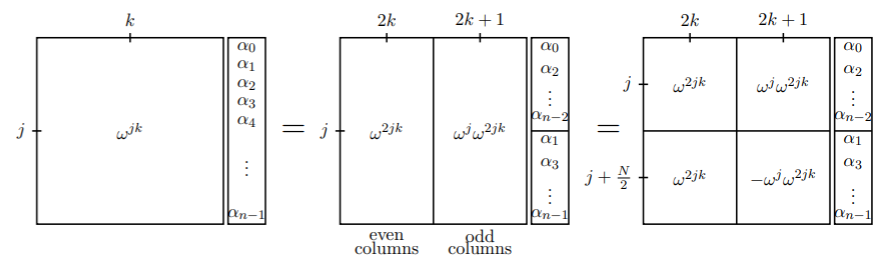
\includegraphics[width=\textwidth]{Images/FFT_8.png}
    \caption{Recursive decomposition of the FFT of size 8}
    \label{fig:FFT_8}
\end{figure}
As shown in Figure~\ref{fig:FFT_8}, the first frame represents the full DFT matrix with entries $\omega_N^{jk}$. The second frame splits the matrix into even and odd columns and separates the input vector accordingly. This leads to a reordering of the DFT matrix as:

\[
QFT_3 = \frac{1}{\sqrt{8}} \begin{pmatrix}
1 & 1 & 1 & 1 & 1 & 1 & 1 & 1 \\
1 & \omega_8^2 & \omega_8^4 & \omega_8^6 & \omega_8 & \omega_8^3 & \omega_8^5 & \omega_8^7 \\
1 & \omega_8^4 & 1 & \omega_8^4 & \omega_8^2 & \omega_8^6 & \omega_8^2 & \omega_8^6 \\
1 & \omega_8^6 & \omega_8^4 & \omega_8^2 & \omega_8^3 & \omega_8 & \omega_8^7 & \omega_8^5 \\
1 & 1 & 1 & 1 & \omega_8^4 & \omega_8^4 & \omega_8^4 & \omega_8^4 \\
1 & \omega_8^2 & \omega_8^4 & \omega_8^6 & \omega_8^5 & \omega_8^7 & \omega_8 & \omega_8^3 \\
1 & \omega_8^4 & 1 & \omega_8^4 & \omega_8^6 & \omega_8^2 & \omega_8^6 & \omega_8^2 \\
1 & \omega_8^6 & \omega_8^4 & \omega_8^2 & \omega_8^7 & \omega_8^5 & \omega_8^3 & \omega_8
\end{pmatrix}
\]

We further use the identity $\omega_N^{j + N/2} = -\omega_N^j$ (since $\omega_N^{N/2} = -1$) to exploit additional symmetry.

\paragraph{Recursive Formula for Functions:} For a function $f(x)$ sampled at $N = 2^n$ points, its DFT $\hat{f}(j)$ can be computed recursively as:

\begin{equation}
    \hat{f}(j) = (F_{N/2} \vec{f}_{\text{even}})(j) + \omega_N^j \cdot (F_{N/2} \vec{f}_{\text{odd}})(j),
\end{equation}

where $F_{N/2}$ denotes the $DFT_{N/2}$ operator, and $\vec{f}_{\text{even}}$, $\vec{f}_{\text{odd}}$ are the even and odd indexed components of the input vector $\vec{f}$, respectively.

Thus, computing $DFT_N$ can be reduced to two $DFT_{N/2}$ operations. Continuing this recursive breakdown leads to four $DFT_{N/4}$ computations, and so on, until we reach $DFT_1 = 1$. Since there are $\log_2 N$ recursive levels and each level requires $O(N)$ operations, the total cost is:
\[
T(N) = O(N \log N).
\]
This dramatically simplifies the computation of the Fourier transform and underpins many efficient classical algorithms. Let us now see an application of FFT.

To figure how to implement the QFT, ket's look at some examples of QFT matrices for a few different sizes.
\begin{equation}
    QFT_1=H=\frac{1}{\sqrt{2}}\begin{bmatrix}\omega^0 & \omega^0\\
    \omega^0 & \omega^1 \end{bmatrix}=\frac{1}{2} \begin{bmatrix}
        1 & 1 \\
        1 & -1
    \end{bmatrix}
\end{equation}
\begin{equation}
    QFT_2 = \frac{1}{2}\begin{bmatrix}
        1 & 1 & 1 & 1 \\
        1 & \omega & \omega^2 & \omega^3\\
        1 & \omega^2 & \omega^0 & \omega^2 \\
        1 & \omega^3 & \omega^6 & \omega^9
    \end{bmatrix}=
        \frac{1}{2} \begin{bmatrix}
            1 &1 & 1 & 1\\
            1 & \omega & \omega^2 & \omega^3\\
            1 & \omega^2 & \omega^0 & \omega^2\\
            1 & \omega^3 & \omega^2 & \omega^1
        \end{bmatrix}=\frac{1}{2}\begin{bmatrix}
            1 & 1 & 1 & 1\\
            1 & \iota & -1 & -\iota \\
            1 & -1 & 1 & -1 \\
            1 & -\iota & -1 & \iota 
        \end{bmatrix}
\end{equation}
\begin{equation}
    QFT_3= \frac{1}{\sqrt{8}} \begin{pmatrix}
1 & 1 & 1 & 1 & 1 & 1 & 1 & 1 \\
1 & \omega_8^2 & \omega_8^4 & \omega_8^6 & \omega_8 & \omega_8^3 & \omega_8^5 & \omega_8^7 \\
1 & \omega_8^4 & 1 & \omega_8^4 & \omega_8^2 & \omega_8^6 & \omega_8^2 & \omega_8^6 \\
1 & \omega_8^6 & \omega_8^4 & \omega_8^2 & \omega_8^3 & \omega_8 & \omega_8^7 & \omega_8^5 \\
1 & 1 & 1 & 1 & \omega_8^4 & \omega_8^4 & \omega_8^4 & \omega_8^4 \\
1 & \omega_8^2 & \omega_8^4 & \omega_8^6 & \omega_8^5 & \omega_8^7 & \omega_8 & \omega_8^3 \\
1 & \omega_8^4 & 1 & \omega_8^4 & \omega_8^6 & \omega_8^2 & \omega_8^6 & \omega_8^2 \\
1 & \omega_8^6 & \omega_8^4 & \omega_8^2 & \omega_8^7 & \omega_8^5 & \omega_8^3 & \omega_8
\end{pmatrix}
\end{equation}
As in equation, the $\omega$'s in the examples above are the $N$th roots of unity where $N$ is the dimension of the matrix. We could design an algorithm to apply these matrices by brute force, but there's a better way. This method is related to one of the most widely used classical algorithms, the Fast Fourier Transform or FFT.

Suppose we have a vector of length $N$, and we want to apply a $N\times N$ matrix $A$ to it. In general this requires us to do the full matrix-vector multiplication which takes $N^2$. However, if we know that $A$ is the Fourier transform, then the FFT lets us apply it in only $O(N\log_2 N)$ steps, by exploring regularities in the Fourier matrix.

What regularity is there in the Fourier matrix? Look at $QFT_2$. If we swap the second and third columns, we get:
\[
\frac{1}{2}\begin{bmatrix}
    1 & 1 & 1 & 1 \\
    1 & \iota & -1 & -\iota \\
    1 & -1 &1 & -1 \\
    1 & -\iota & -1 & \iota
\end{bmatrix}\rightarrow \frac{1}{2}\begin{bmatrix}
    1 & 1 & 1 & 1 \\
    1 & -1 & \iota & -\iota \\
    1 & 1 & -1 & -1 \\
    1 & -1 & -\iota & \iota
\end{bmatrix}
\]
Notice how the matrix can be broken up into 4 blocks, each either equal to $H$ or related to $H$ by the application of a diagonal matrix. In fact if we define the matrix $B$ as
\[
B=\begin{bmatrix}
    1 & 0\\
    0 & \iota
\end{bmatrix}
\]
then we can rewrite the transformed $QFT_2$ matrix above as
\[
\frac{1}{\sqrt{2}}\begin{bmatrix}
    H & BH \\
    H & -BH
\end{bmatrix}
\]
You can do a similar procedure for $QFT_3$, moving all the odd columns to the left and the even columns to the right. Simplifying the $\omega$'s, we get,
\[
\frac{1}{2\sqrt{2}}\begin{pmatrix}
1 & 1 & 1 & 1 & 1 & 1 & 1 & 1 \\
1 & \omega_8^2 & \omega_8^4 & \omega_8^6 & \omega_8 & \omega_8^3 & \omega_8^5 & \omega_8^7 \\
1 & \omega_8^4 & 1 & \omega_8^4 & \omega_8^2 & \omega_8^6 & \omega_8^2 & \omega_8^6 \\
1 & \omega_8^6 & \omega_8^4 & \omega_8^2 & \omega_8^3 & \omega_8 & \omega_8^7 & \omega_8^5 \\
1 & 1 & 1 & 1 & \omega_8^4 & \omega_8^4 & \omega_8^4 & \omega_8^4 \\
1 & \omega_8^2 & \omega_8^4 & \omega_8^6 & \omega_8^5 & \omega_8^7 & \omega_8 & \omega_8^3 \\
1 & \omega_8^4 & 1 & \omega_8^4 & \omega_8^6 & \omega_8^2 & \omega_8^6 & \omega_8^2 \\
1 & \omega_8^6 & \omega_8^4 & \omega_8^2 & \omega_8^7 & \omega_8^5 & \omega_8^3 & \omega_8
\end{pmatrix}
\]
which we can rewrite as
\[
\frac{1}{\sqrt{2}}\begin{bmatrix}
    QFT_2 & B QFT_2\\
    QFT_2 & -BQFT_2
\end{bmatrix}
\]
where the $B$ matrix is now given by
\[
B=\begin{bmatrix}
    1 & 0 & 0 & 0 \\
    0 & \omega & 0 & 0 \\
    0 & 0 & \omega^2 & 0\\
    0 & 0& 0 &  \omega^3
\end{bmatrix}
\]
You can work out why it happens on your own, but it turns out that we can define $QFT_N$ in terms of this nesting recurrence:
\[
QFT_n = \frac{1}{\sqrt{2}}\begin{bmatrix}
    QFT_{n-1} & B_{n-1} F_{n-1}\\
    F_{n-1} & -B_{n-1}QFT_{n-1}
\end{bmatrix}
\]
where we've now defined the generalization of the diagonal $B$ matrix above, $B_{n-1}$ as (omitting the zero on the off-diagonal)
\[
\begin{bmatrix}
    1 & & & & \\
    & \omega & & & \\
    &&\omega^2 &&\\
    &&&\ddots &\\
    &&&&\omega^{2^n-1}
\end{bmatrix}
\]
If we let $C(QFT_n)$ be the number of steps needed to apply $QFT_n$, we get the recurrence relation
\[
C(QFT_n)\leq 2C(QFT_{n-1})+O(N)
\]
for which the solutions is $C(QFT_n)=O(N\log_2 N)$.

In the quantum case, we're actually interested in the unitary transformation $\ket{\psi}\rightarrow QFT_n\ket{\psi}$, where $\ket{\psi}$ is a quantum state of $\log_2 N$ qubits. In one sense, our new goal is less ambitious since we don't need the result vector written explicitly in memory anywhere; it only needs to be encoded implicitly in a vector of amplitudes. In another sense, though, our new goal is more ambitious, since we now want to apply a Fourier transform in time polynomial in only $\log_2 N$.

So how do we do it? we can use the same recursion that we used for the FFT, plus the additional observation that the recursion behaves ``linearly" with respect to the quantum states. Let's think of our $\log_2N$ qubits as representing an integer from $0$ to $N-1$ in binary notation and let's order the bits of that integer from most to least signifcant. But let's also reorder the bits, so that the one that was previously the least significant is now the most significant (the analogue of reordering the columns in our recursion for $QFT_n$). Then we can try applying the circuit $QFT_{n-1}$ to the ``first hair" of the number. In other words, we apply $QFT_{n-1}$ to all but (now) most significant bit. This corresponds to applying the matrix (in block notation)
\[
I_2 \otimes QFT_{n-1} = \begin{bmatrix}
    QFT_{n-1} & 0 \\ 
    0 & QFT_{n-1}
\end{bmatrix}
\]
To get a $B$ in the bottom right quadrant, we can apply a controlled-$B$ gate using the most significant as the control. A controlled-$B$ gate can be written in the form
\[
\begin{bmatrix}
    I & 0 \\
    0 & B
\end{bmatrix}
\]
So after we apply the controlled-$B$ gate, we have
\[
\begin{bmatrix}
    I & 0 \\
    0 & B
\end{bmatrix}
\begin{bmatrix}
    QFT_{n-1} & 0\\0 & QFT_{n-1}
\end{bmatrix}= \begin{bmatrix}
    QFT_{n-1} & 0 \\
    0 & QFT_{n-1}
\end{bmatrix}
\]
We can implement $B$ using a linear number of gates, because it simply amounts to the following:
\begin{itemize}
    \item If the most significant bit is $1$, then do a rotation by some angle $\theta$.
    \item If the second bit is $1$, then do a rotation that's half as big
    \item If the third bit is $1$, then do a rotation that's a quarter as big
    \item etc...
\end{itemize}
By the time you reach the last couple of bits, the rotation is exponentially small. The final steps to get the matrix we want is a Hadamard gate applied to the most significant bit,
\[
H\otimes I_{n-1} = \frac{1}{\sqrt{2}}\begin{bmatrix}
    I_{n-1} & I_{n-1}\\
    I_{n-1} & -I_{n-1}
\end{bmatrix}
\]
which results in the final matrix
\[
\frac{1}{\sqrt{2}}\begin{bmatrix}
    I & I \\
    I & -I
\end{bmatrix}\begin{bmatrix}
    QFT_{n-1} & 0\\0& BQFT_{n-1}
\end{bmatrix} = \begin{bmatrix}
    QFT_{n-1} & BQFT_{n-1}\\
    QFT_{n-1} & -BQFT_{n-1}
\end{bmatrix}
\]
The complete circuit for recursively implementing the Quantum Fourier transform is as shown in figure~\ref{fig:qft_contrs_decom}.


\noindent \textbf{Application: multiplying two polynomials}\\
Suppose we are given two real-values polynomials $p$ and $q$, each of degree at most $d$:
\[
p(x)=\sum_{j=0}^d a_jx^j \quad \text{and} \quad q(x)=\sum_{k=0}^{d} b_kx^k
\]
We would like to compute the product of these two polynomials, which is
\[
(p\cdot q)(x)=\left(\sum_{j=0}^{d}a_jx^j\right)\left(\sum_{k=0}^d b_kx^k\right)=\sum_{l=0}^{2d}(\sum_{j=0}^{2d}a_jb_{l-j})x^l
\]
where implicitly we set $a_j=b_j=0$ for $j>d$ and $b_{l-j}=0$ if$j>l$. Clearly, each coefficient $c_l$ by itself takes $O(d)$ steps (additions and multiplications) to compute, which suggest and algorithm for computing the coefficients of $p\cdot q$ takes $O(d^2)$ steps. However, using the fast Fourier transform we can do this in $O(d\log_2 d)$ steps, as follows.

The convolution of two vectors $a,b\in\mathbb{R}^N$ is a vector $a*b\in\mathbb{R}^N$ whose $l$-th entry is defined by $(a*b)_l=\frac{1}{\sqrt{N}}\sum_{j=0}^{N-1}a_jb_{l-j\mod N}$. Let us set $N=2d+1$ (the number of nonzero coefficients of $p\cdot q$) and make the above $(d+1)$-dimensional vectors of coefficients $a$ and $b$ N-dimensional y addition $d$ zeroes. Then the coefficients of the polynomial $p\cdot q$ are proportional to the entries of the convolution: $c_l=\sqrt{N}(a*b)_l$. It is easy to show that the Fourier coefficients of the convolution of $a$ and $b$ are the products of the Fourier coefficients of $a$ and $b$: for every $l\in\{0,\ldots,N-1\}$ we have $(\hat{a*b})_l=\hat{a}_l*\hat{b}_l$. This immediately suggests an algorithm for computing the vector of coefficients $c_l$: apply the FFT to $a$ and $b$ to get $\hat{a}$ and $\hat{b}$, multiply those two vectors entry wise to get $\hat{a*b}$, apply the inverse FFT to get $a*b$, and finally multiply $a*b$ with $\sqrt{N}$ to get the vector $c$ of the coefficients of $p\cdot q$. Since the FFTs and their inverse take $O(N\log_2 N)$ steps, and point wise multiplication of two $N$-dimensional vectors takes $O(N)$ steps, this algorithm takes $O(N\log_2N)=O(d\log_2d)$ steps.

Note that if two numbers $a_d \ldots a_1a_0$ and $b_d\ldots b_1b_0$ are given in decimal notation, then we can interpret their digits as coefficients of single-variate degree-$d$ polynomials $p$ and $q$, respectively: $p(x)=\sum_{j=0}^d a_jx^j$ and $q(x)=\sum_{k=0}^d b_kx^k$. The two numbers will now be $p(10)$ and $q(10)$. Their product is the evaluation of the product polynomial $p\cdot q$ at the point $x=10$. This suggests hat we use the above procedure (for fast multiplication of polynomials) to multiple two numbers in $O(d\log_2d)$ steps which would be a lot faster than th standard $O(d^2)$ algorithm for multiplication that one learns in primary school. However, in this case we have to be careful since the steps of the above algorithm are themselves multiplication between numbers, which we cannot count at unit cost anymore if our goal is to implement a multiplication between numbers! Sill, it turns out that implementing this idea carefully allows one to multiply two $d$-digit numbers in $O(d\log_2 d\log_2 \log_2 d)$ elementary operations. This is known as the Schohage-Strassen algorithm (slightly improved by Furer and Harey and van der Hoeven), and is one of the ingredients of Shor's algorithm).

\subsubsection{Quantum Fourier Transform (QFT)}

The Quantum Fourier Transform (QFT), sometimes also referred to as the Quantum Fast Fourier Transform (QFFT), is the quantum analogue of the Discrete Fourier Transform (DFT). We will assume $N = 2^n$. In this case, the transformation corresponds to an $n$-qubit unitary operation.

Unlike the classical DFT, where we are given a vector $\vec{x}$ and compute $\vec{y} = DFT_N \vec{x}$ explicitly on classical memory, the QFT operates on quantum states. These quantum states exist only as amplitudes of a superposition, and we cannot access them directly; rather, we apply unitary transformations that act on the amplitudes.

The QFT can be implemented as a quantum circuit using $O(n^2)$ elementary quantum gates. While this is exponentially faster in terms of gate complexity compared to the classical FFT, which requires $O(N \log_2 N) = O(n 2^n)$ operations, the QFT achieves something fundamentally different: it encodes the Fourier transform into the amplitudes of the output quantum state, not into a classical list of coefficients. Hence, the result cannot be directly observed or written down, but can be leveraged in quantum algorithms such as Shor’s algorithm, where the QFT is used as a subroutine.

\section{Quantum Fourier Transform}
\begin{definition}[Quantum Fourier Transform]
The \textit{Quantum Fourier Transform (QFT)} is mathematically identical to the classical Discrete Fourier Transform (DFT), although the conventional notation in the quantum setting is somewhat different. The \textit{quantum Fourier transform} on an orthonormal basis \( \{ \ket{0}, \ket{1}, \dots, \ket{N-1} \} \) is defined to be a linear operator with the following action on the basis states:
\begin{equation}
    \ket{j} \mapsto \frac{1}{\sqrt{N}} \sum_{k=0}^{N-1} e^{2\pi\iota jk / N} \ket{k}.
    \label{eq:qft}
\end{equation}

Equivalently, the action of the QFT on an arbitrary quantum state can be expressed as:
\begin{equation}
    \sum_{j=0}^{N-1} x_j \ket{j} \mapsto \sum_{k=0}^{N-1} y_k \ket{k},
    \label{eq:qft_full}
\end{equation}
where the coefficients \( y_k \) are precisely the Discrete Fourier Transform of the amplitudes \( x_j \), as defined earlier in Equation~\eqref{eq:dft}.

Since the QFT performs the same linear transformation as the DFT, its matrix representation is exactly the same as that of the DFT. From this point onward, we denote the Quantum Fourier Transform matrix by \( \text{QFT}_N \), and treat it as identical to \( \text{DFT}_N \).
\end{definition}


\subsection{Properties of the Quantum Fourier Transform (QFT)}

\subsubsection{QFT is Unitary}

\begin{theorem}
The Quantum Fourier Transform matrix \( \text{QFT}_N \) is unitary, i.e.,
\begin{equation}
    \text{QFT}_N^\dagger \, \text{QFT}_N = I_N.
\end{equation}
\end{theorem}

\begin{proof}
To show that \( \text{QFT}_N \) is unitary, we must prove that its columns are orthonormal. Let \( C_i \) and \( C_j \) denote the \( i \)th and \( j \)th columns of \( \text{QFT}_N \), respectively. Then,
\begin{equation}
    \braket{C_i | C_j} = \frac{1}{N} \sum_{k=0}^{N-1} \omega_N^{-ik} \cdot \omega_N^{jk} = \frac{1}{N} \sum_{k=0}^{N-1} \omega_N^{(j - i)k}.
\end{equation}
If \( i = j \), by equation~\eqref{eq:trivial_sum} this sum becomes
\[
    \sum_{k=0}^{N-1} 1 = N \quad \Rightarrow \quad \braket{C_i | C_i} = 1.
\]
If \( i \neq j \), then the sum forms a geometric series:
\begin{equation}
    \sum_{k=0}^{N-1} \omega_N^{(j - i)k} = \frac{1 - \omega_N^{(j - i)N}}{1 - \omega_N^{(j - i)}} = 0,
\end{equation}
since \( \omega_N^N = 1 \), implying \( \omega_N^{(j - i)N} = 1 \). Therefore by equation~\eqref{eq:sum_powers_of_omega},
\[
    \braket{C_i | C_j} = 0 \quad \text{for } i \neq j.
\]
This confirms that the columns of \( \text{QFT}_N \) are orthonormal:
\[
    \braket{C_i | C_j} = \delta_{ij}.
\]
Hence, \( \text{QFT}_N \) is a unitary matrix.
\end{proof}

Because the Quantum Fourier Transform is a unitary operation, it can be implemented as a quantum circuit. When \( N = 2^n \), the QFT acts on an \( n \)-qubit quantum register.

   \subsubsection{Linear Shift Invariance}

\begin{theorem}[Linear Shift Induces Phase Shift]
Let \( \ket{\psi} \) be a quantum state with Fourier transform \( \ket{\phi} \). We say that a state vector $\ket{\psi} =\sum_{j=0}^{N-1} \psi_j \ket{j}$ has been linearly shifted by an integer $m$ when we obtain the state $\ket{\psi'} = \sum_{j=0}^{N-1} \psi_{j'} \ket{j}$ where $j' = (j+m)\mod N$. Let the action of QFT operator on $\ket{\beta}$ and $\ket{\beta'}$ (shifted state) results in $\ket{\beta}$ and $\ket{\beta'}$ respectively. Then the components of $\ket{\beta'}$ in the computational basis differ by the respective components of $\ket{\beta}$ by a phase i.e.
\begin{equation}
\beta_k' =\omega_N^{-km}\cdot \beta_k
\end{equation}
where $\omega_N=e^{2\pi\iota /N}$.
\end{theorem}
\begin{proof}
    Let \( \text{QFT}_N \) (identical to \( \text{DFT}_N \)) be the normalized Fourier matrix of size \( N \), given by:
\begin{equation}
    (\text{QFT}_N)_{jk} = \frac{1}{\sqrt{N}} \, \omega_N^{jk}, \quad \text{where } \omega_N = e^{2\pi\iota / N}.
\end{equation}

Let the quantum state be represented as \( \ket{\psi} = \begin{bmatrix}
    \psi_0 &\psi_1 & \ldots & \psi_{N-1} 
\end{bmatrix}^\top\). Then its Fourier-transformed state is:
\begin{equation}
    \ket{\beta} = \text{QFT}_N \ket{\psi}, \quad \text{where } \beta_k = \frac{1}{\sqrt{N}} \sum_{j=0}^{N-1} \omega_N^{jk} \psi_j.
\end{equation}
Here, $\beta_k$ is the $k$th component of the quantum state $\ket{\beta}$.
Now consider a linearly shifted version of the state by \( m \) positions:
\[
    \ket{\psi'} = \begin{bmatrix}
        \psi_m & \psi_{m+1} & \ldots & \psi_{(N+m-1 \mod N)}
    \end{bmatrix}^\top
\]
Then the Fourier transform of \( \ket{\psi'} \) results in \(\ket{\beta'}\) whose $k$th component is given as,
\begin{equation}
    \beta_k' = \frac{1}{\sqrt{N}} \sum_{j=0}^{N-1} \omega_N^{kj} \psi_{(j+m \mod N)} = \omega_N^{-km} \frac{1}{\sqrt{N}} \sum_{j=0}^{N-1} \omega_N^{k(j+m)} \psi_{(j+m \mod N)}\\
\end{equation}
Using the periodicity property of powers of $N$th primitive root of unity as given in equation~\eqref{eq:periodicity}, we get, 
\begin{align*}
    \beta_k' &= \omega_N^{-km} \left(\frac{1}{\sqrt{N}} \sum_{j=0}^{N-1} \omega_N^{k(j+m \mod N)} \psi_{(j+m \mod N)}\right)\\
    &=\omega_N^{-km}\left(\frac{1}{\sqrt{N}}\sum_{p = (m \mod N)}^{N+m-1\mod N}\omega_N^{kp}\psi_{p}\right)
\end{align*}
Since there are $N$ terms in the expansion and the iterator $j$ iterates over all the possible values from $j=0,\ldots,N-1$, so does the iterator $p = (j+m \mod N)$ will iterate over. Thus, it can be simplified as,
\begin{equation}
    \beta_k' = \omega_N^{-km}\left( \frac{1}{\sqrt{N}} \sum_{j=0}^{N-1} \omega_N^{kj}\psi_{j}\right) = \omega_N^{-km}\cdot \beta_k
\end{equation}
Thus, a linear shift introduces a global phase factor \( \omega_N^{-km} \) to each Fourier coefficient. 
\end{proof}
This does not affect measurement outcomes, as:
\[
    |\beta_k'|^2 = |\omega_N^{-km} \beta_k|^2 = |\beta_k|^2.
\]
Consider the following demonstration for more clarity.
\begin{example}[QFT Under Linear Shift]
Let \( N = 4 \), and define:
\[
\ket{\theta} = 
\begin{pmatrix}
    \alpha_0 \\
    \alpha_1 \\
    \alpha_2 \\
    \alpha_3
\end{pmatrix}, \quad
\ket{\phi} = 
\begin{pmatrix}
    \alpha_1 \\
    \alpha_2 \\
    \alpha_3 \\
    \alpha_0
\end{pmatrix}.
\]

Then the Fourier transform matrices yield:
\begin{align*}
    \text{QFT}_4 \ket{\theta} &= \frac{1}{2}
    \begin{pmatrix}
        1 & 1 & 1 & 1 \\
        1 & i & -1 & -i \\
        1 & -1 & 1 & -1 \\
        1 & -i & -1 & i
    \end{pmatrix}
    \begin{pmatrix}
        \alpha_0 \\
        \alpha_1 \\
        \alpha_2 \\
        \alpha_3
    \end{pmatrix} =
    \begin{pmatrix}
        \beta_0 \\
        \beta_1 \\
        \beta_2 \\
        \beta_3
    \end{pmatrix}, \\
    \text{QFT}_4 \ket{\phi} &= \frac{1}{2}
    \begin{pmatrix}
        1 & 1 & 1 & 1 \\
        1 & i & -1 & -i \\
        1 & -1 & 1 & -1 \\
        1 & -i & -1 & i
    \end{pmatrix}
    \begin{pmatrix}
        \alpha_1 \\
        \alpha_2 \\
        \alpha_3 \\
        \alpha_0
    \end{pmatrix} =
    \begin{pmatrix}
        \beta_0' \\
        \beta_1' \\
        \beta_2' \\
        \beta_3'
    \end{pmatrix}.
\end{align*}
Note that here the components \(\beta_k\) are given as,
\begin{align*}
    \beta_0 &= \frac{1}{2}(\alpha_0+\alpha_1+\alpha_2+\alpha_3)\\
    \beta_1 &= \frac{1}{2}(\alpha_0+\iota\alpha_1-\alpha_2-\iota\alpha_3)\\
    \beta_2 &=\frac{1}{2}(\alpha_0-\alpha_1+\alpha_2-\alpha_3)\\
    \beta_3 &=\frac{1}{2}(\alpha_0 -\iota \alpha_1 -\alpha_2+\iota\alpha_3)
\end{align*}
We now compute each component \( \beta_k' \) and verify the phase relationships:
\begin{align*}
\beta_0' &= \frac{1}{2}(\alpha_1+\alpha_2+\alpha_3+\alpha_0) = \frac{1}{2}(\alpha_0+\alpha_1+\alpha_2+\alpha_3)=\beta_0\\
    \beta_1' &= \frac{1}{2} (\alpha_1 + \iota\alpha_2 - \alpha_3 - \iota\alpha_0) = -\iota \cdot \frac{1}{2} (\alpha_0 + \iota\alpha_1 - \alpha_2 - \iota\alpha_3) = -\iota \beta_1, \\
    \beta_2' &= \frac{1}{2} (\alpha_1 - \alpha_2 + \alpha_3 - \alpha_0)
    = -1 \cdot \frac{1}{2} (\alpha_0 - \alpha_1 + \alpha_2 - \alpha_3) = -\beta_2, \\
    \beta_3' &= \frac{1}{2} (\alpha_1 - \iota\alpha_2 - \alpha_3 + \iota\alpha_0)
    = \iota \cdot \frac{1}{2} (\alpha_0 - \iota\alpha_1 - \alpha_2 + \iota\alpha_3) = \iota \beta_3.
\end{align*}

Thus, the linear shift induces the phase transformation:
\[
\beta_0'=\beta_0,\quad  \beta_1' = -\iota \beta_1, \quad \beta_2' = - \beta_2, \quad \beta_3' = \iota \beta_3.
\]
which shows that $\beta_k' = e^{2\pi\iota k/4}\cdot \beta_k$.
\end{example}
\begin{remark}
Thus, if we are going to measure a state, then the phases don't matter at all as $|e^{\iota \theta}|=1$. Therefore the phase of a given state does not effect the probability of measuring the state. While these phase shifts change the relative amplitudes, they do not affect the measurement probabilities. Since the modulus \( |e^{i\theta}| = 1 \), the probability of observing each basis state remains unchanged. Therefore, quantum measurement is insensitive to global or relative phase shifts introduced by quantum Fourier transforms of linearly shifted states.
\end{remark} 

In order to gather information about the phases, consider the following example.
\begin{example}
    Consider the states $\ket{\theta}=\frac{1}{2}\begin{pmatrix} 1 \\ 1 \\ 1 \\ 1 \end{pmatrix}$ and $\ket{\phi}=\frac{1}{2}\begin{pmatrix} 1 \\ \iota \\ -1 \\ -\iota \end{pmatrix}$. 
        We can't tell the difference by measuring the states.
        Upon applying $QFT_2$. We get:
        \[ QFT_2\ket{\theta}=\begin{pmatrix} 1 \\ 0 \\ 0 \\ 0 \end{pmatrix} \]
        \[ QFT_2\ket{\phi}=\begin{pmatrix} 0 \\ 1 \\ 0 \\ 0 \end{pmatrix} \]
        Thus, measuring the Fourier Transform of the states will reveal the relative phases. Note that this was because the transformation induces a relative phase shift on each Fourier component but preserves the probability amplitudes:
\[
|\beta_k'|^2 = |\beta_k|^2.
\]
\end{example}        


\subsubsection{Period and Wavelength Relationship} 
\begin{theorem}
Suppose $\ket{\psi}$ is a quantum state. We apply the Quantum Fourier Transform (QFT) to this function, which is essentially the Discrete Fourier Transform (DFT) over $N=2^n$ points:
\[
QFT_n \ket{\psi} = \ket{\beta},
\]
where $\ket{\beta}$ denotes the Fourier transform of $\ket{\psi}$. Then \textbf{period} of $\ket{\psi}$ is the smallest positive integer $r$ such that:
\[
\psi_{i} = \psi_{(i\mod r)}, \quad \forall i=0,\ldots,N-1.
\]
The \textbf{wavelength} of $\ket{\beta}$ is the smallest positive integer $s$ such that:
\[
\beta_i=\beta_{(i \mod s)}, \quad \forall i=0,\ldots,N-1. 
\]
These two are related by:
\[
s = \frac{N}{r}.
\]
Thus, the number of repetitions (or frequency peaks) in the Fourier domain is inversely proportional to the periodicity in the original domain.
\end{theorem}
\begin{proof}
In matrix form, this can be expressed as:
\[
\frac{1}{\sqrt{N}}\begin{pmatrix} 
1 & 1 & 1 & \cdots & 1 \\
1 & \omega_N & \omega_N^2 & \cdots & \omega_N^{N-1} \\
1 & \omega_N^2 & \omega_N^4 & \cdots & \omega_N^{2(N-1)} \\
\vdots & \vdots & \vdots & \ddots & \vdots \\
1 & \omega_N^{N-1} & \omega_N^{2(N-1)} & \cdots & \omega_N^{(N-1)^2}
\end{pmatrix}
\begin{pmatrix}
\psi_0 \\ \psi_1 \\ \psi_2 \\ \vdots \\ \psi_{r-1} \\ \psi_0 \\ \psi_1 \\ \vdots
\end{pmatrix}
=
\begin{pmatrix}
\beta_0 \\ \beta_1 \\ \beta_2 \\ \vdots \\ \beta_{s-1} \\ \beta_0 \\ \beta_1 \\ \vdots
\end{pmatrix},
\]
where $\omega_N = e^{2\pi\iota/N}$ is the $N$-th primitive root of unity.

This relationship is visually represented in Figure~\ref{fig:QFT_Period_Wavelength}.
We can write the output for $k=1,\ldots,N-1$ as,
\begin{align*}
\beta_k &= \frac{1}{\sqrt{N}}\sum_{j=0}^{N-1} \omega_N^{jk} \psi_{j \text{ mod } r}\\
&=\frac{1}{\sqrt{N}}\left(\sum_{j=0}^{r-1}\omega_N^{jk}\psi_j + \sum_{j=0}^{r-1} \omega_N^{(j+r)k}\psi_j + \ldots \sum_{j=0}^{r-1} \omega_N^{(j+(\frac{N}{r}-1)r)k}\psi_j\right)\\
&=\frac{1}{\sqrt{N}}\left(\sum_{j=0}^{r-1}\omega_N^{jk}\psi_j + \omega_N^{rk}\sum_{j=0}^{r-1} \omega_N^{jk}\psi_j + \ldots+ \omega_N^{(\frac{N}{r}-1)rk} \sum_{j=0}^{r-1} \omega_N^{jk}\psi_j\right)\\
&=\frac{1}{\sqrt{N}}\left(\sum_{j=0}^{r-1}\omega_N^{jk}\psi_j\right)\left(\sum_{p=0}^{\frac{N}{r}-1} \omega_N^{prk}\right)
\label{eq:simplification_period}
\end{align*}
Now, the geometric series $\sum_{p=0}^{\frac{N}{r}-1}\omega_N^{prk}$ simplifies as follows:
\[
\sum_{p=0}^{\frac{N}{r}-1} \omega_N^{prk}=
\begin{cases}
    \frac{N}{r}, &\text{if $k\equiv 0 \mod \frac{N}{r}$}\\
    0, &\text{else}
\end{cases}
\]
Now recall that $k=0,\ldots,N-1$. This evaluates the equation to
\[
\frac{1}{\sqrt{N}} \sum_{j=0}^{r-1}\omega_N^{jk}\psi_j\left(\sum_{p=0}^{N/r} \omega_N^{prk}\right) = \begin{cases}
    \frac{1}{\sqrt{N}}\frac{N}{r}\sum_{j=0}^{r-1}\omega_N^{jk}\psi_j &\text{if $k\equiv 0 \mod \frac{N}{r}$}\\
    0 &\text{else}
\end{cases} 
\]

\begin{figure}[ht]
    \centering
    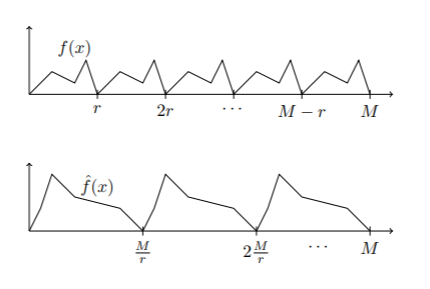
\includegraphics[width=0.7\textwidth]{Images/QFT_period_wavelength.png}
    \caption{Relationship between period $r$ in the time domain and wavelength $s = \frac{2^n}{r}$ in the frequency domain.}
    \label{fig:QFT_Period_Wavelength}
\end{figure}

\noindent
In general, the sharper (more localized) the function in the time domain, the more spread out it is in the Fourier domain, and vice versa. For instance, the Fourier transform of a delta function is a uniform spread, whereas that of a uniform spread is a delta function.    
\end{proof}


\begin{example}[Periodic Delta Function]
Consider a function defined as:
\[
f(x) = 
\begin{cases}
\sqrt{\frac{r}{2^n}} & \text{if } x \equiv 0 \pmod{r}, \\
0 & \text{otherwise}.
\end{cases}
\]
\begin{figure}[ht]
    \centering
    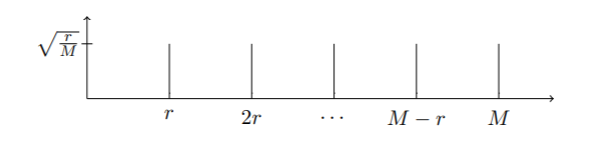
\includegraphics[width=0.6\textwidth]{Images/f(x).png}
    \caption{Periodic function $f(x)$}
    \label{fig:f(x)}
\end{figure}
For our $f(x)$:
\[
f(x) = 
\begin{cases}
\sqrt{\frac{r}{N}} & \text{if } x \equiv 0 \pmod{r}, \\
0 & \text{otherwise},
\end{cases}
\]
we compute:
\[
\hat{f}(x) = \frac{\sqrt{r}}{N} \sum_{i=0}^{\frac{N}{r}-1} \omega_N^{r i x}.
\]
This is a geometric sum. Using the formula:
\[
\sum_{i=0}^{N-1} z^i = \frac{1 - z^N}{1 - z},
\]
we obtain:
\[
\hat{f}(x) = \frac{\sqrt{r}}{2^n} \cdot \frac{1 - \omega_N^{rx \cdot N}}{1 - \omega^{rx}}.
\]
Since $\omega_N^{N} = 1$, the numerator becomes zero. So when $rx \equiv 0 \pmod{N}$, both numerator and denominator are zero. Apply L’Hôpital’s Rule:
\[
\lim_{x \rightarrow q\frac{N}{r}} \frac{1 - \omega_N^{x N}}{1 - \omega_N^{rx}} 
= \lim_{x \rightarrow q\frac{N}{r}} \frac{-N \omega_N^{xN}}{-r \omega_N^{rx}} 
= \frac{N}{r}.
\]
Substituting back gives:
\[
\hat{f}(x) = 
\begin{cases}
\frac{1}{\sqrt{r}} & \text{if } x \equiv 0 \pmod{\left(\frac{N}{r}\right)}, \\
0 & \text{otherwise}.
\end{cases}
\]
This is the type of function used in Shor’s algorithm to identify periodicity. Refer to Figures~\ref{fig:f(x)} and~\ref{fig:QFT_f(x)}.
\begin{figure}[ht]
    \centering
    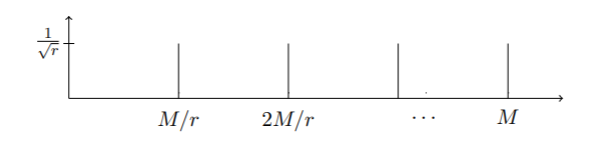
\includegraphics[width=0.6\textwidth]{Images/QFT_f(x).png}
    \caption{QFT of $f(x)$}
    \label{fig:QFT_f(x)}
\end{figure}
This result shows that periodic functions transform into sparse Fourier spectra with well-defined peaks. More generally, any function with period $r$ can be expressed as a linear combination of such basis functions, possibly with phase shifts. This is what is use in Shor's algorithm.
\end{example}

\begin{remark}
The Discrete Fourier Transform maps a vector
\begin{equation}
    \ket{\alpha} = \begin{pmatrix} \alpha_0 \\ \alpha_1 \\ \vdots \\ \alpha_{N-1} \end{pmatrix}
\end{equation}
into a new vector
\begin{equation}
    \ket{\beta} = \begin{pmatrix} \beta_0 \\ \beta_1 \\ \vdots \\ \beta_{N-1} \end{pmatrix}, \quad \text{where } \beta_k = \frac{1}{\sqrt{N}} \sum_{j=0}^{N-1} \omega_N^{kj} \alpha_j.
    \label{eq:fourier_transform_formula}
\end{equation}
This transformation spreads or compresses the distribution depending on the original vector's structure as we saw in the properties of the QFT matrix based on the relation between period and wavelength of a function.
\end{remark}

\subsection{Examples and Applications of the QFT}
Now we will see a few example demonstrations of properties of QFT Matrix.
\begin{example}[QFT for $N=2$ and $N=4$]
For $N = 2$, we have $\omega_2 = -1$, and the QFT matrix becomes:
\[
    QFT_2 = \frac{1}{\sqrt{2}}\begin{pmatrix} 1 & 1 \\ 1 & -1 \end{pmatrix},
\]
which is exactly the Hadamard matrix $H$.

For $N = 4$, $\omega_4 = i$, and we get:
\begin{equation}
    QFT_2 = \frac{1}{2} \begin{pmatrix}
        1 & 1 & 1 & 1 \\
        1 & i & -1 & -i \\
        1 & -1 & 1 & -1 \\
        1 & -i & -1 & i
    \end{pmatrix}.
    \label{eq:qft4_matrix}
\end{equation}
\end{example}
\begin{example}
Transform the quantum state $\ket{\psi} = \frac{1}{\sqrt{2}} (\ket{0} + \ket{3})$ using $QFT_2$.
Let $\omega_4 = e^{2\pi\iota / 4} = i$. Then,
\begin{equation}
    QFT_2 = \frac{1}{2}\begin{pmatrix}
        1 & 1 & 1 & 1 \\
        1 & i & -1 & -i \\
        1 & -1 & 1 & -1 \\
        1 & -i & -1 & i
    \end{pmatrix},
    \label{eq:f4_matrix}
\end{equation}
and
\[
    \ket{\psi} = \frac{1}{\sqrt{2}} \begin{bmatrix} 1 \\ 0 \\ 0 \\ 1 \end{bmatrix}.
\]
Applying $QFT_2$:
\[
    QFT_2 \ket{\psi} = \frac{1}{2\sqrt{2}} \begin{bmatrix} 2 \\ 1 - i \\ 0 \\ 1 + i \end{bmatrix} = \frac{1}{2\sqrt{2}}(2\ket{0} + (1 - i)\ket{1} + (1 + i)\ket{3}).
\]
\end{example}
\begin{example}[DFT Action on Simple States]
Let
\[
    \ket{f} = \frac{1}{2} \begin{pmatrix} 1 \\ 1 \\ 1 \\ 1 \end{pmatrix}, \quad
    \ket{g} = \ket{0} = \begin{pmatrix} 1 \\ 0 \\ 0 \\ 0 \end{pmatrix}, \quad
    \ket{h} = \ket{1} = \begin{pmatrix} 0 \\ 1 \\ 0 \\ 0 \end{pmatrix}.
\]
Then:
\begin{align*}
    QFT_2 \ket{f} &= \frac{1}{4}\begin{pmatrix} 1 & 1 & 1 & 1 \\ 1 & i & -1 & -i \\ 1 & -1 & 1 & -1 \\ 1 & -i & -1 & i \end{pmatrix} \begin{pmatrix} 1 \\ 1 \\ 1 \\ 1 \end{pmatrix} = \begin{pmatrix} 1 \\ 0 \\ 0 \\ 0 \end{pmatrix}, \\
    QFT_2 \ket{g} &= \frac{1}{2} \begin{pmatrix} 1 \\ 1 \\ 1 \\ 1 \end{pmatrix}, \\
    QFT_2 \ket{h} &= \frac{1}{2} \begin{pmatrix} 1 \\ i \\ -1 \\ -i \end{pmatrix}.
\end{align*}
Note:
\begin{itemize}
    \item The columns of $QFT_2$ are orthonormal, confirming unitarity.
    \item The state $\ket{f}$ is uniform (flat), and its Fourier transform is sharply peaked as demonstrated in the relation between period and wavelength.
    \item $\ket{g}$ and $\ket{h}$ differ in phase in the frequency domain which demonstrates the property of Phase Shift under Linear Shift.
\end{itemize}
\end{example}

We shall now demonstrate how to implement quantum Fourier transform efficiently using quantum gates.

\section{Efficient implementation of Quantum Fourier Transform}
Here's some intuition on how the Fourier transform works. In graduate school you can easily fall into a 26-hour-per-day cycle. So, one day you wake up at 8am, the next day you wake up at 10am then 12pm, and so forth so that if nothing interrupts you, you cycle all the way around. Suppose you've fallen into such a cycle and you want to figure out how long the cycle is without doing any complicated calculations like subtraction.

What you can do is install a series of clocks in your room, each tracking ``days" of different lengths. So, you'd have a 23-hour clock, a 24-hour clock, a 25-hour clock, etc.. In addition, you install a bulletin board below each clock and place a single thumbstack in its center. Now, every time you wake up you go to each clock and move the thumbstack one inch in the direction the hour hand points.

What will happen if you keep doing this, week after week? If you're really keeping 26-hour days, then the thumbstack corresponding to the 26-hour clock will always move in the same direction. This is constructive interference! And the same is true for the 13-hour clock (as well as the 1-hour and 2-hour clocks). All the others - the 23-hour clock, the 24-hour clock, etc. will have the thumbstack move around, sometimes in one direction, sometimes another, so that it eventually returns to the origin.

The Quantum Fourier transform is essentially this, but with quantum amplitudes instead of thumbstacks. Recall that the Quantum Fourier Transform (QFT) is essentially a unitary matrix (identical to DFT). So the question is how to implement the Quantum Fourier Transform using a small quantum circuit. Recall that not all unitaries are efficiently implementable so it's not obvious that a $N\times N$ matrix can be implemented using a circuit with only $polylog(N)$ gates.
\subsection{Idea of the Algorithm}
The strength of the FFT is that we are able to use the symmetry of the discrete Fourier transform to our advantage.
The circuit application of QFT uses the same principle, but because of the power of superposition QFT is even faster.

The QFT is motivated by the FFT so we will follow the same steps, but because this is a quantum algorithm the implementation of the steps will be different. 
We first take the Fourier transform of the odd and even parts, then multiply the odd terms by the phase $\omega^j$.

In quantum algorithm, the first step is that the odd and even terms are together in superposition: the odd terms are those 
whose least significant bit is 1, and even with 0. Therefore, we can apply $QFT_{n-1}$ to both the odd and even terms together.
We do this by simply applying the $QFT_{n-1}$ to the n-1 most significant bits, and recombine the odd and even appropriately by 
applying the Hadamard to the least significant bit as shown in the figure~\ref{fig:qft_decompose_circ}
\begin{figure}[ht]
    \centering
    \begin{quantikz}
        \lstick[3]{$n-1$ qubits}& \gate[4]{QFT_n} & \\
        & & \\
        \vdots \\
        \lstick[1]{least significant bit}& & 
    \end{quantikz}$\rightarrow$\begin{quantikz}
        & \gate[2]{QFT_{n-1}} & &\\
        & & &\\
        \vdots \\
        & & \gate{H} &
    \end{quantikz}
    \caption{$QFT_{n-1}$ and a Hadamard gate correspond to $DFT_{n-1}$} on the odd and even terms.
    \label{fig:qft_decompose_circ}
\end{figure}
Now to carry out the phase multiplication, we need to multiply each odd term j by the phase $\omega_j$. But remember, an odd number in binary ends with a 1, while an even ends with 0.
Thus, we can use the controlled phase shift, where the least significant bits is the control, to multiply only the odd terms by the phase without doing anything to the even terms. 
Recall that the controlled phase shift is similar to the CNOT gate in that it only applies a phase to the target if the control bit is one.

The phase associated with each controlled phase shift should be equal to $\omega^j$ where j is associated to the kth bit by $j=2^k$.
Thus, apply the controlled phase shift to each of the first $n-1$ qubits , with the least significant bit as the control. 
With the controlled phase shift and the Hadamard transform, $QFT_n$ has been reduced to $QFT_{n-1}$ as shown in the figure~\ref{fig:qft_contrs_decom}.
\begin{figure}[ht]
    \centering
    \begin{quantikz}
        \lstick[4]{$n-1$ qubits} & \gate[5]{QFT_{n}} & \\
        & & \\
        & & \\
        \vdots \\
        \lstick[1]{least significant bit} & & 
    \end{quantikz}=\begin{quantikz}
        & \gate[3]{QFT_{n-1}} &  & \gate{P_2} & & & \\
        & & & & \gate{P_3} & & \\
        & & & & & \gate{P_4}& \\
        \vdots \\
        & & \gate{H} & \ctrl{-4} & \ctrl{-3} & \ctrl{-2} & & \\
    \end{quantikz}
    \caption{$QFT_n$ is reduced to $QFT_{n-1}$ and $n$ additional gates}
    \label{fig:qft_contrs_decom}
\end{figure}
\begin{example}
    Let us construct $QFT_3$. Following the algorithm, we will turn $QFT_4$ into $QFT_3$ and a few quantum gates. Then continuing on this way we turn $QFT_3$ into $QFT_1$ (which is just a Hadamard gate) and another few gates.
    Controlled phase gates will be represented by $P_{k}$. \textbf{Number of gates necessary to carry out $QFT_n$ is exactly $\sum_{i=1}^{\log N}i=\log N(\log N+1)/2=O(\log^2 N)$.}
    Thus, the circuit is as shown in the figure \ref{fig:Qft_iteration}.
    \begin{figure}[ht]
        \centering
        \begin{quantikz}
            \lstick[1]{$\ket{x_2}$} & \gate[2]{QFT_2} & \gate{P_3} & & & \\
            \lstick[1]{$\ket{x_1}$} & & & \gate{P_2} & & \\
            \lstick[1]{$\ket{x_0}$} & & \ctrl{-2} & \ctrl{-1} & \gate{H} & 
        \end{quantikz}$\rightarrow$ \begin{quantikz}
            \lstick[1]{$\ket{x_2}$} & \gate{H}\gategroup[2,steps=3,style={dashed,rounded corners, , inner xsep=2pt},background,label style={label position=above, anchor=south, yshift=-0.2cm}]{{\sc $QFT_2$}} & \gate{P_2}& & \gate{P_3} & & & \\
            \lstick[1]{$\ket{x_1}$} & & \ctrl{-1}& \gate{H} & & \gate{P_2} & & \\
            \lstick[1]{$\ket{x_0}$} & & & &  \ctrl{-2} & \ctrl{-1} & \gate{H} &
        \end{quantikz}
        \caption{First and second iteration. Recall that $QFT_1=H$}
        \label{fig:Qft_iteration}
    \end{figure}
\end{example}

\subsection{Intuitive way}
To get a feeling of how this works, let's first consider the case where $n=3$. For each $j\in\{0,1\}^3=\{0,1,2,3,4,5,6,7\}$, the corresponding Fourier basis state $QFT_3\ket{j}$ is
\[
\frac{1}{\sqrt{8}}(\ket{000}+\omega_8^j\ket{001}+\omega_8^{2j}\ket{010}+\omega_8^{3j}\ket{011}+\omega_8^{4j}\ket{100}+\omega_8^{5j}\ket{101}+\omega_8^{6j}\ket{110}+\omega_8^{7j}\ket{111})
\]
A natural question to ask is are these three qubits entangled or can be decomposed into a tensor product state? The answer is, yes, they are in a product state. In fact, this state can be written as
\begin{align*}
\frac{1}{\sqrt{8}}\ket{0}\otimes(\ket{00}+\omega_8^j\ket{01}&+\omega_8^{2j}\ket{10}+\omega_8^{3j}\ket{11})+ \\
&\omega_8^{4j}\ket{1}\otimes(\ket{00}+\omega_8^{j}\ket{01}+\omega_8^{2j}\ket{10}+\omega_8^{3j}\ket{11})\\
&=\frac{1}{\sqrt{8}}(\ket{0}+\omega_8^{4j}\ket{1})\otimes (\ket{00}+\omega_8^j\ket{01}+\omega_8^{2j}\ket{10}+\omega_8^{3j}\ket{11})\\
&=\frac{1}{\sqrt{8}}(\ket{0}+\omega_8^{4j}\ket{1})\otimes(\ket{0}+\omega_8^{2j}\ket{1})\otimes (\ket{0}+\omega_8^j\ket{1})
\end{align*}
So $QFT_3\ket{j}$ is a tensor product of three $1$-qubit states. This generalizes to $QFT_n\ket{j}$ for all $n\geq 1$, as follows.
\begin{lemma}\label{lem:QFT}
    For all $n\geq1$ and $j\in\{0,1\}^n$
    \begin{equation}
        QFT_n\ket{j} = \frac{1}{\sqrt{2^{n}}}(\ket{0}+\omega_N^{2^{n-1}j}\ket{1})\otimes \ldots \otimes (\ket{0}+\omega_N^{4j}\ket{1})\otimes (\ket{0}+\omega_N^{2j}\ket{1})\otimes (\ket{0}+\omega_N^j\ket{1})
        \label{eq:qft_n}
    \end{equation}
\end{lemma}
Our quantum circuit for computing the Fourier transform will make use of this structure. Remember that, if we compute a linear operator that matches the Fourier transform on all computational basis states then it must be the Fourier transform.

Let's return our attention to the $n=3$ case, where the Fourier basis states are
\begin{equation}
QFT_3\ket{j}=\frac{1}{\sqrt{8}}(\ket{0}+\omega_8^{4j}\ket{1})\otimes(\ket{0}+\omega_8^{2j}\ket{1})\otimes (\ket{0}+\omega_8^j\ket{1})
\label{eq:qft_8}
\end{equation}
for all $j\in\{0,1\}^3$. Each $j=j_2j_1j_0$ denotes the element of $\{0,1,2,3,4,5,6,7\}$ in the usual way ($j_0$ is the lower-order bit and $j_2$ is the high-order bit).

Consider the state of the first qubit in equation~\eqref{eq:qft_8}. Since $\omega^4=-1$, the state of the first qubit simplifies to $\ket{0}+(-1)^j\ket{1}$. Note that this is $\ket{+}$ when $j$ is even and $\ket{-}$ when $j$ is odd. The parity of $j$ is determined by its lower-order bit $j_0$. Therefore the first qubit of $QFT_3\ket{j}$ is simply $H\ket{j_0}$.

What about the remaining qubits. Let $\ket{\psi}$ denote the second and third qubit in equation~\eqref{eq:qft_8}. That is,
\begin{equation}
\ket{\psi}=\frac{1}{\sqrt{4}}(\ket{0}+\omega_8^{2j}\ket{1})\otimes (\ket{0}+\omega_8^j\ket{1})
\label{eq:psi_2q}
\end{equation}
Now, please look at the $n=2$ case of the expression in equation~\eqref{eq:qft_n}. Does $\ket{\psi}$ look like $QFT_2\ket{j}$?

There is a certainly superficial resemblance; however $\ket{\psi}$ and $QFT_2\ket{j}$ are not exactly the same. The state $QFT_2\ket{j}$ is with respect to a $4$th root of unity - not an $8$th root of unity. Another difference is that $QFT_2$ acts on $2$ qubits; whereas the parameter $j$ in equation~\eqref{eq:psi_2q} is a $3$-bit integer.

It will be fruitful to explore in more detail the difference between $\ket{\psi}$ and $QFT_2\ket{j}$. Let's see what these state look like in terms of the digits $j_2j_1j_0$ of the binary representation of $j$. We'll use the Greek letter $\omega_4$ to denote the $4$th root of unity, while reserving $\omega_8$ for the $8$th root of unity.

If we apply $QFT_2$ to $\ket{j_2j_1}$ (the two higher order bits of $j$), the result is
\begin{align*}
    QFT_2\ket{j_2j_1} &=\frac{1}{\sqrt{4}}(\ket{0}+\omega_4^{2(j_2j_1)_2}\ket{1})\otimes(\ket{0}+\omega_4^{(j_2j_1)_2}\ket{1})\\
    &=\frac{1}{\sqrt{4}}(\ket{0}+(\omega_8^2)^{2(j_2j_1)_2}\ket{1})\otimes(\ket{0}+(\omega_8^2)^{(j_2j_1)_2}\ket{1})\\
    &=\frac{1}{\sqrt{4}}(\ket{0}+\omega_8^{2(j_2j_10)_2}\ket{1})\otimes (\ket{0}+\omega_8^{(j_2j_10)_2}\ket{1})
\end{align*}
In the exponent, I've surrounded the binary representations by brackets so that they can be clearly read; the two-digit number in the brackets is either $0,1,2,$ or $3$. The above has been derived from Lemma~\ref{lem:QFT} and we have use the property that $\omega_4=\omega_8^2$. And in the last step we have simply used the binary equivalent of what we do in base ten when we multiply an integer by ten: we add a zero digit and shift all the other digits left. 10 times 23 is 230.

Now let's express $\ket{\psi}$ in terms of $(j_2j_1j_0)_2$. This is
\begin{align*}
    \ket{\psi}&=\frac{1}{\sqrt{4}}(\ket{0}+\omega_8^{2(j_2j_1j_0)_2}\ket{1})\otimes(\ket{0}+\omega_8^{(j_2j_1j_0)_2}\ket{1})\\
    &=\frac{1}{\sqrt{4}}(\ket{0}+\omega_8^{2(j_2j_10)_2}\omega_8^{2j_0}\ket{1})\otimes (\ket{0}+\omega_8^{j_2j_10)_2}\omega_8^{j_0}\ket{1})
\end{align*}
Comparing the two equation $QFT_2\ket{j}$ and $\ket{\psi}$, we can see precisely where they differ: the factors $\omega_8^{2j_2}$ and $\omega_8^{j_2}$. We'll refer to these as phase corrections.

Based on the above observations, let's try to compute $QFT_3\ket{j_0j_1j_2}$ in terms of $QFT_2\ket{j_1j_2}$ and $H\ket{j_0}$, combined with additional gates that perform phase corrections. To perform the phase corrections, we introduce the $2$-qubit controlled-phase gate $CP_k$ as follows:
\[
CP_k = \begin{bmatrix}
    I & 0 \\ 0 & P_k 
\end{bmatrix}=\begin{bmatrix}
    1 & 0 & 0 & 0 \\
    0 & 1 & 0 & 0 \\
    0 & 0 & 1 & 0 \\
    0 & 0 & 0 & e^{2\pi\iota /2^k}
\end{bmatrix}
\]
where $P_k=\begin{bmatrix}
    1 & 0 \\
    0 & e^{2\pi\iota/2^k}
\end{bmatrix}$.
Now we'll analyze the circuit as shown in figure~\ref{fig:decomp_qft_8} and show that it computes $QFT_3$.
\begin{figure}[ht]
    \centering
    \begin{quantikz}[slice all]
        \lstick[1]{$\ket{j_2}$} & \gate[2]{QFT_2} & & \gate{P_2} & & &\swap{1} & \\
        \lstick[1]{$\ket{j_1}$} & & \gate{P_3} & & & \swap{1}& \targX{} &\\
        \lstick[1]{$\ket{j_0}$} & & \ctrl{-1} & \ctrl{-2} & \gate{H} & \targX{} & &
    \end{quantikz}=\begin{quantikz}
        &\gate[3]{QFT_3}&\\
        & & \\
        & &
    \end{quantikz}
    \caption{Decomposition of $QFT_3$}
    \label{fig:decomp_qft_8}
\end{figure}
We will now trace through the stages of this circuit.\\
\textbf{At stage 1:}\\
We know that $QFT_2\ket{j}$ will be $\frac{1}{\sqrt{4}}(\ket{0}+\omega_8^{2(j_2j_10)_2}\ket{1})\otimes (\ket{0}+\omega_8^{(j_2j_10)_2}\ket{1})$.\\
\textbf{After stage 2 and 3:}\\
The two controlled-phase gate changes the state to
\begin{align*}
    \frac{1}{\sqrt{4}}(\ket{0}+\omega_8^{2(j_2j_10)_2}&\omega_8^{2j_0}\ket{1})\otimes (\ket{0}+\omega_8^{(j_2j_10)_2}\omega_8^{j_0}\ket{1})\otimes \ket{j_0}\\
    &=\frac{1}{\sqrt{4}}(\ket{0}+\omega_8^{2(j_2j_1j_0)_2}\ket{1})\otimes(\ket{0}+\omega_8^{(j_2j_1j_0)_2}\ket{1})\otimes \ket{j_0}\\
    &=\frac{1}{\sqrt{4}}(\ket{0}+\omega_8^{2j}\ket{1})\otimes (\ket{0}+\omega_8^j\ket{1})\otimes \ket{j_0}
\end{align*}
\textbf{At stage 4:}\\
Applying the Hadamard gate to the third qubit changes the state to
\begin{align*}
    \frac{1}{\sqrt{4}}(\ket{0}+\omega_8^{2j}\ket{1})\otimes &(\ket{0}+\omega_8^j\ket{1})\otimes\frac{1}{\sqrt{2}}(\ket{0}+(-1)^{j_0}\ket{1})\\
    &=\frac{1}{\sqrt{8}}(\ket{0}+\omega_8^{2j}\ket{1})\otimes (\ket{0}+\omega_8^j\ket{1})\otimes(\ket{0}+\omega_8^{4j}\ket{1})
\end{align*}
Notice that this is the state in equation~\eqref{eq:qft_8}, except the qubits are in the wrong order.\\
\textbf{At stage 5 and 6:}\\
Moving the third qubit to the left and shifting the other two qubits right yields
\[
(\ket{0}+\omega^{4j}\ket{1})\otimes(\ket{0}+\omega^{2j}\ket{1})\otimes (\ket{0}+\omega^j\ket{1})=QFT_3\ket{j}
\]
What we have shown is a special case of the following more general recurrence for $QFT_n$. 
\begin{lemma}\label{lem:qft_constr}
    For all $n\geq 1$, The Fourier transform $QFT_n$ can be expressed as in figure~\ref{fig:qft_const}.
    \begin{figure}[ht]
        \centering
        \begin{quantikz}
            & \gate[6]{QFT_n} &\\
            & &\\
            \vdots\\
            & & \\
            & &\\
            &&
        \end{quantikz}=\begin{quantikz}
            & \gate[5]{QFT_{n-1}} & &&\ \ldots \ &&\gate{P_2}&&&&\swap{1} &\\
            & & && \ \ldots \ &\gate{P_3}&&&&&\targX{} &\\
            \vdots \\
            & &&\gate{P_{n-1}}&\ \ldots \ &&&& &\swap{1} & &&\\
            &&\gate{P_n}&&\ \ldots \ &&&& \swap{1} &\targX{} &&\\
            &&\ctrl{-1}&\ctrl{-2}& \ \ldots \ & \ctrl{-4} &\ctrl{-5}&\gate{H}&\targX{} & & &
        \end{quantikz}
        \caption{Quantum circuit for $QFT_n$ recursively construed in terms of $QFT_{n-1}$}
        \label{fig:qft_const}
    \end{figure}
\end{lemma}

By repeatedly applying lemma~\ref{lem:qft_constr}, we can construct quantum circuit for the Fourier transform for any $n\geq1$. The recurrence bottoms out at $n=1$, where $QFT_2=H$. Notice that there are places where the qubits are rearranged. Instead of doing these rearrangements, we can move the gates around. Then there's just one net arrangement at the very end, which turns out to be a reversal of the order of the qubits which can be done using SWAP gates. For example, look at the circuit for the case of $n=4$ as shown in figure~\ref{fig:qft_exn4}.
\begin{figure}[ht]
    \centering
    \scalebox{0.75}{\begin{quantikz}
        & \gate{H} & \gate{P_2} & \gate{P_3} & \gate{P_4}& & & & &&&&\swap{3}&&\\
        & & \ctrl{-1} & & & \gate{H} & \gate{P_2} & \gate{P_3} & &&&&& \swap{1}&\\
        & & & \ctrl{-2} & & & \ctrl{-1} & & \gate{H} & \gate{P_2} & &  & & \targX{} & \\
        & & & & \ctrl{-3} & & & \ctrl{-2} & & \ctrl{-1} & & \gate{H} & \targX{} & &
    \end{quantikz}}
    \caption{Quantum Circuit for $QFT_2$, with rearrangements deferred until the end}
    \label{fig:qft_exn4}
\end{figure}


\subsection{Mathematical Way}
We will now go in a more mathematically rigorous manner proving for the general case.
For any computational basis $\ket{j}$, recall that $N=2^n$ Fourier transform is defined as,
\[
QFT_n\ket{j}=\frac{1}{\sqrt{N}}\sum_{k=0}^{N-1} e^{\iota 2\pi \frac{kj}{N}}\ket{k}
\]
for $j=0,\ldots,N-1$. Also action of quantum Fourier transform on $\ket{0^n}$ is same as Hadamard applied to each qubit as shown,
\[
QFT_n\ket{0^n}=\frac{1}{\sqrt{N}}\sum_{k=0}^{N-1}\ket{k}=H^{\otimes n}\ket{0^n}
\]
Inverse Fourier transform is then defined by taking its conjugate (since $QFT_n^{\dagger}QFT_n=I=QFT_nQFT_n^{\dagger} \implies QFT_n^{\dagger}=QFT_n^{-1}$) for any computational basis $\ket{k}$ as:
\begin{equation}
QFT_n^{\dagger}\ket{k}=\frac{1}{\sqrt{N}}\sum_{j=0}^{N-1}e^{-\iota 2\pi \frac{kj}{N}}\ket{j}
\label{eq:inv_qft}
\end{equation}
Note that $QFT_n^{\top}=QFT_n$. Thus, $QFT_n^{\dagger}=(QFT_n^\top)^*=QFT_n^*$.

We will adopt the \textit{big-endian} notation throughout this chapter, i.e., the most significant bit (MSB) is assigned to the highest index, and the least significant bit (LSB) to the lowest. Specifically, for any integer \( k \in \{0, \dots, 2^n - 1\} \), we write its binary representation as
\[
k = (k_{n-1} \ldots k_0)_2,
\]
where \( k_{n-1} \) is the most significant bit and \( k_0 \) is the least significant bit.
Let us now represent $k,j$ in binary representation. Then
\[
k=(k_{n-1}\ldots k_0)_2, \quad j=(j_{n-1}\ldots j_0)_2
\]
Thus, 
\[
k=k_{n-1}2^{n-1}+\ldots+k_0; \quad j=j_{n-1}2^{n-1}+\ldots +j_0
\]
We have
\begin{align*}
\frac{kj}{2^n}&=\frac{1}{2^n}(k_{n-1}2^{n-1}+\ldots+k_0)j\\
&=\left(\frac{k_{n-1}}{2}+\ldots+\frac{k_0}{2^n}\right)j\\
&=\frac{k_{n-1}j}{2}+\ldots+\frac{k_0j}{2^n}\\
&=\frac{k_{n-1}}{2}\left(j_{n-1}2^{n-1}+\ldots +j_0\right)+\ldots + k_0\left(j_{n-1}2^{n-1}+\ldots +j_0\right)\\
&=k_{n-1}(j_{n-1}2^{n-2}+\ldots+\frac{j_0}{2})+\ldots +k_0(j_{n-1}2^{n-1}+\ldots+j_0)\\
&=k_{n-1}(j_{n-1}\ldots j_1.j_0)_2+\ldots +k_0(0.j_{n-1}\ldots j_0)_2\\
\end{align*}
Thus we have simplified $\frac{kj}{2^n}$ as,
\begin{equation}
    \frac{kj}{2^n}=k_0(0.j_{n-1}\ldots j_0)_2+\ldots +k_{n-1}(j_{n-1}\ldots j_1.j_0)_2
    \label{eq:kjN}
\end{equation}
Thus, substituting in the exponential $e^{\iota 2\pi \frac{kj}{2^n}}$ can be written as
\begin{align*}
    e^{\iota 2\pi \frac{kj}{2^n}}&=e^{\iota 2\pi k_0(0.j_{n-1}\ldots j_0)_2+\ldots +k_{n-1}(j_{n-1}\ldots j_1.j_0)_2}\\
    &=e^{\iota 2\pi k_0(0.j_{n-1}\ldots j_0)_2}\cdot \ldots \cdot e^{\iota 2\pi k_{n-1}(j_{n-1}\ldots j_1.j_0)_2}
\end{align*}
Thus, now using the fact that $e^{\iota 2\pi k(p.q)_2}=e^{\iota 2 \pi k (p+0.q)_2}=e^{\iota 2 \pi kp}e^{\iota 2 \pi k(0.q)_2}=e^{\iota 2 \pi k (0.q)_2}$ for integer $p$, as $e^{2\pi\iota kp}=1$.
\begin{align*}
    QFT_n\ket{j_{n-1}\ldots j_0} &=\frac{1}{\sqrt{N}}\sum_{k_{n-1},\ldots ,k_0}(e^{\iota 2\pi (k_0(0.j_{n-1}\ldots j_0)_2}\ldots e^{\iota 2\pi k_{n-1}(j_{n-1}\ldots j_1.j_0)_2})\ket{k_{n-1}\ldots k_0}\\
    &=\frac{1}{\sqrt{N}}\sum_{k_{n-1},\ldots ,k_0}(e^{\iota 2\pi k_{n-1}(0.j_0)_2}\ldots e^{\iota 2\pi (k_0(0.j_{n-1}\ldots j_0)_2})\ket{k_{n-1}\ldots k_0}\\
    &=\frac{1}{\sqrt{N}}\sum_{k_{n-1},\ldots ,k_0}(e^{\iota 2\pi k_{n-1}(0.j_0)_2}\ket{k_{n-1}}\otimes \ldots \otimes e^{\iota 2\pi (k_0(0.j_{n-1}\ldots j_0)_2}\ket{k_0})\\
    &=\frac{1}{\sqrt{N}}\sum_{k_{n-1},\ldots,k_0} \bigotimes_{l={n-1}}^0 e^{\iota 2 \pi k_l(0.j_{l-n+1}\ldots j_0)_2}\ket{k_l}\\
    &=\frac{1}{\sqrt{N}}\left(\sum_{k_{n-1}=0}^1 e^{\iota 2 \pi k_{n-1}(0.j_0)_2}\ket{k_{n-1}}\right)\otimes \left(\sum_{k_{n-2}=0}^1 e^{\iota 2 \pi k_{n-2} (0.j_1j_0)_2}\ket{k_{n-2}}\right) \otimes \ldots \otimes \\
    &\quad \left(\sum_{k_0=0}^1 e^{\iota 2 \pi k_0(0.j_{n-1}\ldots j_0)_2}\ket{k_0}\right)\\
    &=\frac{1}{\sqrt{N}} \bigotimes_{l={n-1}}^0 \left( \sum_{k_l=0}^1 e^{\iota 2 \pi k_l(0.j_{l-n+1}\ldots j_0)_2}\ket{k_l}\right)\\
    \implies QFT_n\ket{j_{n-1}\ldots j_0} &=\left(\frac{\ket{0}+e^{\iota 2 \pi (0.j_0)_2}\ket{1}}{\sqrt{2}}\right)\otimes \left(\frac{\ket{0}+e^{\iota 2 \pi (0.j_1j_0)_2}\ket{1}}{\sqrt{2}}\right) \otimes \ldots \otimes \\
    &\quad \left(\frac{\ket{0}+e^{\iota 2 \pi (0.j_{n-1}\ldots j_0)_2}\ket{1}}{\sqrt{2}}\right)
\end{align*}
Thus, we need to implement manipulations of the form
\[
\ket{j_l}\rightarrow \frac{1}{\sqrt{2}}\left(\ket{0}+e^{\iota 2 \pi (0.j_{n-1-l)}\ldots j_0)_2}\ket{1}\right)
\]
for $l=0,\ldots,n-1$.
using controlled rotations. Note that,
\[
e^{\iota 2 \pi (0.j_{n-1}\ldots j_0)_2}=e^{\iota 2\pi (0.j_{n-1})_2}e^{\iota 2 \pi (0.0j_{n-2})_2}\ldots e^{\iota 2 \pi (0.0\ldots 0j_0)_2}
\]
which can be done by implementing controlled rotations in sequence. Recall the Phase gate
\[
    P({\theta})=\begin{bmatrix}
        1 & 0 \\
        0 & e^{i\theta}
        \end{bmatrix}
\]
Putting $P_l=P(\frac{2\pi}{2^{l}})$. In particular, $P_1=Z$. Let us define,
\begin{equation}
P\left(\frac{2\pi}{2^{l}}\right) = \begin{bmatrix} 1 & 0 \\ 0 & e^{\iota 2\pi/2^{l}} \end{bmatrix}=P_l
\label{eq:phase_gate_defn}
\end{equation}
Hence, clearly, $P_l\ket{0}=\ket{0}$ and $P_l\ket{1}=e^{\iota \frac{2\pi}{2^{l}}}\ket{1}$. We will now show how we can achieve the required transformation using controlled rotations.
\subsubsection{Implementation of controlled rotations}
Consider the implementation of
\[
\ket{j_{n-1}}\rightarrow \frac{1}{\sqrt{2}}\left(\ket{0}+e^{\iota 2\pi (0.j_{n-1}\ldots j_0)_2}\ket{1}\right)
\]
where $\ket{j}=\ket{j_{n-1}\ldots j_0}$. When $n=1$, we need to implement
\[
\ket{j_0}\rightarrow \left(\frac{\ket{0}+e^{\iota 2 \pi (0.j_0)_2}\ket{1}}{\sqrt{2}}\right) = \begin{cases}
    \ket{+}=\frac{\ket{0}+\ket{1}}{\sqrt{2}}, &\text{if $j_0=0$}\\
    \ket{-}=\frac{\ket{0}-\ket{1}}{\sqrt{2}},&\text{if $j_0=1$}
\end{cases}
\]
This is the Hadamard gate:
\[
\ket{j_0}\rightarrow H\ket{j_0}
\]
When $n=2$, we wish to implement
\[
\ket{j_1j_0}\rightarrow \frac{1}{\sqrt{2}}\left(\ket{0}+e^{\iota 2 \pi (0.j_0)}\ket{1}\right)\otimes \frac{1}{\sqrt{2}}\left(\ket{0}+e^{\iota 2 \pi (0.j_1j_0)}\ket{1}\right)
\]
Now, consider the implementation of the following circuit in figure \ref{fig:qft_2q}.
\begin{figure}[ht]
    \centering
    \begin{quantikz}
    \lstick[1]{$\ket{j_1}$} & \gate{H} & \gate{P_2}  & & \swap{1} & \rstick[1]{$\ket{0}+e^{\iota 2\pi(0.j_0)_2}\ket{1}$}   \\
    \lstick[1]{$\ket{j_0}$} & & \ctrl{-1} & \gate{H} & \targX{} & \rstick[1]{$\ket{0}+e^{\iota2\pi(0.j_1j_0)_2}\ket{1}$}
    \end{quantikz}
    \caption{$QFT_2$}
    \label{fig:qft_2q}
\end{figure}
\begin{align*}
    \ket{j_1j_0}&\xrightarrow{H \otimes I} \frac{1}{\sqrt{2}}\left(\ket{0}+e^{\iota 2 \pi (0.j_1)}\ket{1}\right)\ket{j_0}\\
\end{align*}
We then apply the controlled $P_2$ (with $\ket{j_0}$ as the control bit). Now, $P_2=P(\pi/2)=P(2\pi/4)$. Say $j_0=1$, we apply $P_2$ to the state, we get,
\begin{align*}
&=\frac{1}{\sqrt{2}}\begin{pmatrix} 1 & 0 \\ 0  & e^{\iota 2 \pi/4} \end{pmatrix}\begin{pmatrix} 1 \\ e^{\iota 2 \pi (0.j_1)_2}\end{pmatrix}\\&=\frac{1}{\sqrt{2}}\begin{pmatrix} 1 \\ e^{\iota 2 \pi (0.j_11)_2} \end{pmatrix}\\
&=\frac{1}{\sqrt{2}}(\ket{0}+e^{\iota 2\pi(0.j_11)_2}\ket{1})\\
\end{align*}
Say $j_0=0$, then controlled phase gate $P_2$ would not be applied and the state remains the same $\frac{1}{\sqrt{2}}\begin{pmatrix}
    1 \\ e^{\iota 2\pi (0.j_10)_2}
\end{pmatrix}=\frac{1}{\sqrt{2}}(\ket{0}+e^{\iota 2\pi(0.j_1)_2}\ket{1})$. In a more compact form, this can be written as,
\begin{align*}
\frac{1}{\sqrt{2}}\begin{pmatrix} 1 \\ e^{\iota 2 \pi (0.j_1 j_0)_2} \end{pmatrix}&=\begin{cases} \frac{1}{\sqrt{2}}(\ket{0}+e^{\iota 2\pi(0.j_11)_2}\ket{1}) & \text{if $j_0=1$} \\ 
\frac{1}{\sqrt{2}}(\ket{0}+e^{\iota 2 \pi (0.j_10)_2}\ket{1}) &\text{if $j_0=0$} \end{cases}\\
\end{align*}
Thus, the final state in simplified form after the action of controlled-Phase gate can be written as,
\[
\frac{1}{\sqrt{2}}(\ket{0}+e^{\iota 2\pi(0.j_1j_0)}\ket{1})\otimes \ket{j_0}
\]
Now applying the Hadamard gate on $\ket{j_0}$and the finally swapping the qubits, we get,
\begin{align*}
    &\xrightarrow{I\otimes H} \left(\frac{1}{\sqrt{2}}(\ket{0}+e^{\iota 2\pi(0.j_1j_0)}\ket{1})\right)\otimes \left(\frac{1}{\sqrt{2}}(\ket{0}+e^{\iota 2 \pi (0.j_0)\ket{1}}\ket{1})\right)\\
    &\xrightarrow{SWAP} \left(\frac{1}{\sqrt{2}}(\ket{0}+e^{\iota 2 \pi (0.j_0)\ket{1}}\ket{1})\right) \otimes \left(\frac{1}{\sqrt{2}}(\ket{0}+e^{\iota 2\pi(0.j_1j_0)}\ket{1})\right)
\end{align*}
Thus, the required result.
In general this can be extended to $n$ qubits as shown through the following quantum circuit in figure ~\ref{fig:qft_N}.
\begin{figure}[ht]
    \centering
    \scalebox{0.8}{\begin{quantikz}
        \lstick[1]{$\ket{j_{n-1}}$} &  \gate{H} & \gate{P_2} & \gate{P_3} & \ \ldots \ & \gate{P_{n-1}} &\gate{P_n} & &  \ \ldots \ & & && \rstick[1]{$\frac{1}{\sqrt{2}}(\ket{0}+e^{2\pi\iota(0,j_{n-1}\ldots j_0)_2}\ket{1})$}\\
        \lstick[1]{$\ket{j_{n-2}}$} & & \ctrl{-1} & & \ \ldots \ && & \gate{H} &  \ \ldots \ && &&\rstick[1]{$\frac{1}{\sqrt{2}}(\ket{0}+e^{2\pi\iota (0.j_{n-2}\ldots j_0)_2}\ket{1})$}\\
        \vdots \\
        \lstick[1]{$\ket{j_1}$} & & & &  \ \ldots \ &\ctrl{-3}&  & & \ \ldots \ &\gate{H} & \gate{P_2} & & \rstick[1]{$\frac{1}{\sqrt{2}}(\ket{0}+e^{2\pi\iota(0.j_1j_0)_2}\ket{1})$} \\
        \lstick[1]{$\ket{j_0}$} & & & & \ \ldots \ &&\ctrl{-4} & &  \ \ldots & & \ctrl{-1} &\gate{H} & \rstick[1]{$\frac{1}{\sqrt{2}}(\ket{0}+e^{2\pi\iota (0.j_0)_2}\ket{1})$}
    \end{quantikz}}
    \caption{$QFT_n$ circuit without the SWAP gates}
    \label{fig:qft_N}
\end{figure}
and then finally swapping, we can get the required result. Similarly, the circuit for inverse Fourier transform can also be implemented. Recall that since $QFT_n$ is a unitary gate, $QFT_n^{-1}=QFT_n^{\dagger}$. Say $QFT_n=U_1U_2\ldots U_r$, then $QFT_n^{-1}=QFT_n^{\dagger}=U_r^{\dagger}U_{r-1}^{\dagger}\ldots U_1^{\dagger}$. For example, for the case $n=2$, the circuit is as shown in the figure \ref{fig:qftinv_2q}.
\begin{figure}[ht]
    \centering
    \begin{quantikz}
        \lstick[1]{$\ket{j_1}$} & \swap{1} & & \gate{P_2^{\dagger}} & \gate{H} & \rstick[1]{$\frac{1}{\sqrt{2}}(\ket{0}+e^{-\iota 2\pi(0.j_0)}\ket{1})$} \\
        \lstick[1]{$\ket{j_0}$} & \targX{} & \gate{H} & \ctrl{-1} & & \rstick[1]{$\frac{1}{\sqrt{2}}(\ket{0}+e^{-\iota 2\pi(0.j_1j_0)}\ket{1})$}
    \end{quantikz}
    \caption{Quantum circuit for inverse Fourier transform $QFT_2^{-1}$}
    \label{fig:qftinv_2q}
\end{figure}
Note that in the figure for the $QFT_n^{-1}$ circuit, $H^{\dagger}=H$ and we would be required to implement $P_l^{\dagger}$ in controlled-phase gates which is the same as controlled-phase gates with negative phase angles i.e. $P_l^{\dagger}=P\left(-\frac{2\pi}{2^l}\right)$.

The final Quantum Fourier Transform (QFT) circuit with the SWAP gates is given as in figure~\ref{fig:qft_N_withswap}.
\begin{figure}[ht]
    \centering
    \scalebox{0.8}{\begin{quantikz}
        \lstick[1]{$\ket{j_{n-1}}$} &  \gate{H} & \gate{P_2} & \gate{P_3} & \ \ldots \ & \gate{P_{n-1}} &\gate{P_n} & &  \ \ldots \ & & & & \swap{4} &  & \rstick[1]{$\frac{1}{\sqrt{2}}(\ket{0}+e^{2\pi\iota (0.j_0)_2}\ket{1})$}\\
        \lstick[1]{$\ket{j_{n-2}}$} & & \ctrl{-1} & & \ \ldots \ && & \gate{H} &  \ \ldots \ && &&  & \swap{2}&  \rstick[1]{$\frac{1}{\sqrt{2}}(\ket{0}+e^{2\pi\iota(0.j_1j_0)_2}\ket{1})$}\\
        \vdots \\
        \lstick[1]{$\ket{j_1}$} & & & &  \ \ldots \ &\ctrl{-3}&  & & \ \ldots \ &\gate{H} & \gate{P_2} & &  & \targX{} & \rstick[1]{$\frac{1}{\sqrt{2}}(\ket{0}+e^{2\pi\iota (0.j_{n-2}\ldots j_0)_2}\ket{1})$} \\
        \lstick[1]{$\ket{j_0}$} & & & & \ \ldots \ &&\ctrl{-4} & &  \ \ldots & & \ctrl{-1} &\gate{H} &\targX{} &  & \rstick[1]{$\frac{1}{\sqrt{2}}(\ket{0}+e^{2\pi\iota(0,j_{n-1}\ldots j_0)_2}\ket{1})$}
    \end{quantikz}}
    \caption{$QFT_n$ circuit with the SWAP gates}
    \label{fig:qft_N_withswap}
\end{figure}
The SWAP operation is simply swapping the first $\ket{j_{n-1}}$ and last $\ket{j_0}$ qubit, second $\ket{j_{n-2}}$ and second-last $\ket{j_1}$ qubit and so on. Thus, we swap $\ket{j_{n-p}}$th qubit with $\ket{j_{p-1}}$th qubit. A total of $\lfloor \frac{n}{2}\rfloor$ swap gate operations. 
\subsection{Implementation of the controlled-phase gates}
Note that a controlled-phase gate is not in standard 2-qubit gate set, thus we now give a decomposition of the controlled-phase gate into single qubit and CNOT gates.

Recall that to implement a controlled-unitary gate $C-U$ where unitary $U$ acts on a single qubit. Then there exist unitary operators $A,B,C$ on a single qubit such that $ABC=I$ and $U=e^{\iota\alpha}AXBXC$ where $\alpha$ is some overall phase factor and $X$ is the Pauli-X (NOT gate) gate.We can then implement a controlled version of that unitary the controlled unitary $C-U$ by controlling the Pauli-X gates controlled by the control bit by changing them into C-NOT gates with the control qubit as the control bit and the target qubit being the target bit. Suppose the control qubit is set. Then the operation $e^{\iota\alpha}AXBXC$ is applied on the second qubit. If, on the other hand, the control qubit is not set, then the operation $ABC=I$ is applied on the second qubit, that is, no change is made. That is, this circuit implements the controlled-$U$ operation. 

Let phase gate $P_k$ be decomposed as $P_k = e^{\iota \alpha}AXBXC$ with $ABC=I$. This can be implemented Taking $\alpha = \frac{\pi}{2^k},A=I, B=R_Z\left(-\frac{\pi}{2^k}\right)$ and $C=R_Z\left(\frac{\pi}{2^k}\right)$. Note that
\begin{align*}
    ABC&=IR_Z\left(-\frac{\pi}{2^k}\right)R_Z\left(\frac{\pi}{2^k}\right)\\
    &=R_Z\left(-\frac{\pi}{2^k}+\frac{\pi}{2^k}\right)\\
    &=R_Z(0)\\
    ABC&=I
\end{align*}
and we get the unitary $U$,
\begin{align*}
    U&=e^{\iota\alpha}AXBXC\\
    &=e^{\iota \frac{\pi}{2^k}} XR_Z\left(-\frac{\pi}{2^k}\right)XR_Z\left(\frac{\pi}{2^k}\right)
\end{align*}
Using the identity $XR_Z(\theta)X = R_Z(-\theta)$ we get,
\begin{align*}
    U &=e^{\iota\frac{\pi}{2^k}} R_Z\left(\frac{\pi}{2^k}\right)R_Z\left(\frac{\pi}{2^k}\right)
\end{align*}
    Using the fact that $R_Z(\alpha)R_Z(\beta)=R_Z(\alpha+\beta)$,
\begin{align*}
    U&=e^{\iota\frac{\pi}{2^k}}R_Z\left(\frac{2\pi}{2^k}\right)\\
    &=e^{\iota\frac{\pi}{2^k}}\begin{bmatrix}e^{-\iota \frac{\pi}{2^k}} & 0 \\ 0 & e^{\iota\frac{\pi}{2^k}}\end{bmatrix}\\
    &=\begin{bmatrix}
        1 & 0 \\ 0 & e^{\iota\frac{2\pi}{2^k}}
    \end{bmatrix}
\end{align*}
Thus, this implements $U=e^{\iota\alpha}AXBXC=P_k$. The circuit shown in figure~\ref{fig:c-p} implements the controlled phase gate $P_k$
\begin{figure}[ht]
    \centering
    \begin{quantikz}
     & \ctrl{1} & & \ctrl{1}& \phase{e^{\iota\frac{\pi}{2^k}}} & \\
     & \targ{} & \gate{R_Z\left(-\frac{\iota\pi}{2^k}\right)} & \targ{} & \gate{R_Z\left(\frac{\iota\pi}{2^k}\right)} & 
    \end{quantikz}
    \caption{Circuit decomposition of controlled-phase gate $P_k$}
    \label{fig:c-p}
\end{figure}

\subsection{Implementation of SWAP gates}
Recall the definition of a SWAP gate $\ket{x}\ket{y}\rightarrow \ket{y}\ket{x}$. We will show that the the $2$-qubit SWAP gate can be implemented by a sequence of three CNOT gates appropriately oriented. Recall the action of CNOT gate on a state $\ket{x}\ket{y}\rightarrow \ket{x}\ket{x\oplus y}$. Consider the following decomposition as shown in figure~\ref{fig:decomp_swap}.
\begin{figure}[ht]
    \centering
    \begin{quantikz}
        &\swap{1} &\\
        & \targX{} & 
    \end{quantikz} = \begin{quantikz}
        &\ctrl{1} & \targ{} & \ctrl{1} &\\
        &\targ{} & \ctrl{-1} & \targ{} &
    \end{quantikz}
    \caption{Decomposition of SWAP gate into 3 CNOT gates}
    \label{fig:decomp_swap}
\end{figure}
We can verify that the decomposition shown in figure~\ref{fig:decomp_swap} works by verifying its action on all the computational basis states. Say the input was $\ket{x}\ket{y}$ where $x,y\in\{0,1\}$, some 2-qubit computational basis state in the swap gate, then the output should be $\ket{y}\ket{x}$. Let us now check whether the decomposition by 3 CNOT gates performs this operation. The action of first CNOT gives:
\[
\ket{x}\ket{y} \rightarrow \ket{x}\ket{x\oplus y}
\]
The action of second CNOT gives
\[
\ket{x}\ket{x\oplus y} \rightarrow \ket{x\oplus x\oplus y} \ket{x\oplus y}
\]
substituting $x\oplus x=0$, we get the state $\ket{y}\ket{x\oplus y}$. The action of the third CNOT gives
\[
\ket{y}\ket{x\oplus y} \rightarrow \ket{y}\ket{x\oplus y \oplus y}
\]
again using the property that $y\oplus y=0$ for $y\in{0,1}$, we get the state $\ket{y}\ket{x}$ which is the desired state. Thus, the action of 3 CNOT gates as appropriately arranged as shown in the figure~\ref{fig:decomp_swap} is same as the SWAP gate.
\[
\ket{x}\ket{y}\rightarrow \ket{y}\ket{x}
\]
Thus, each SWAP gate can be decomposed into three CNOT gates.
\subsection{Total Gate Complexity}The construction itself proves that the quantum Fourier Transform is Unitary, since each gate in the circuit is unitary. The circuit uses for the first qubit 1 Hadamard gate and $n-1$ conditional gates. This is followed by a Hadamard gate and $n-2$ conditional rotations for the second qubit, and so on till the $n$th qubit where we apply only $1$ Hadamard gate. Continuing this way, we see that $n+(n-1)+\ldots + 1$ gates are required, plus the gates involved in the swaps. At most $n/2$ swaps are required, and each swap can be accomplished using three controlled CNOT gates. Also, from the figure, we can clearly see that the total number of gates are $n+n-1+\ldots +1$. This is following the recurrence relation:
\[
g(r+1)=g(r)+r+1;\quad \text{with base case} \quad g(1)=1
\]
which simplifies to,
\[
g(n) = \sum_{j=1}^n j =\binom{n+1}{2}=\frac{n(n+1)}{2}
\]
and including the $\lfloor n/2\rfloor$ swap operations,we get,
\[
\frac{n(n+1)}{2} +\frac{n}{2}=O(n^2)
\]
Thus, $O(n^2)$ gate complexity in total. Therefore, this circuit provides a $O(n^2)=O(\log_2 N \log_2 \log_2N)$ algorithm for performing the $N=2^n$ quantum Fourier Transform.
\section{Quantum Fourier transform when $N$ is prime}
(Analysis to be done)

\section{Approximate Quantum Fourier Transform}
We can reduce the circuit complexity to linear in $\log n$ if we are willing to settle for an implementation of fixed accuracy, because the two-qubit gates acting on distantly separated qubits contribute only exponentially small phases.

Recall the phase gate
\[
P_k = \begin{bmatrix}
    1 & 0 \\
    0 & e^{\frac{2\pi\iota}{2^k}}
\end{bmatrix}
\]
and the unitary corresponding to the controlled phase gate
\[
\begin{bmatrix}
    1 & 0 & 0 & 0 \\
    0 & 1 & 0 & 0 \\
    0 & 0 & 1 & 0 \\
    0 & 0 & 0 & e^{\iota\frac{2\pi}{2^k}}
\end{bmatrix}
\]
Here, the phase is $\frac{2\pi}{2^k}$, so as the value of $k$ increases the value of phase tends to zero. Hence, for higher values of $k$ the controlled Phase gate tends to be identity. Let us now find the error between the controlled phase gate and the Identity gate.
\begin{align*}
\|I_{4} - CP_k\|_2 =\|\begin{bmatrix}
    1 & 0 & 0 & 0 \\
    0 & 1 & 0 & 0 \\
    0 & 0 & 1 & 0 \\
    0 & 0 & 0 & 1 
\end{bmatrix} - \begin{bmatrix}
    1 & 0 & 0 & 0 \\
    0 & 1 & 0 & 0 \\
    0 & 0 & 1 & 0 \\
    0 & 0 & 0 & e^{\iota\frac{2\pi}{2^k}}
\end{bmatrix}\|=\|\begin{bmatrix}
    0 & 0 & 0 & 0 \\
    0 & 0 & 0 & 0 \\
    0 & 0 & 0 & 0 \\
    0 & 0 & 0 & 1-e^{\iota\frac{2\pi}{2^k}}
\end{bmatrix}\|
\end{align*}
Recall that the $2-norm$ of a matrix is the largest singular value of the matrix. In this case, since it's a diagonal matrix, the singular value will correspond to the modulus of the diagonal entries. Thus, out of singular values $0$ with multiplicity $3$ and $|1-e^{\iota\frac{2\pi}{2^k}}|$ with multiplicity $1$, clearly the only contributing singular value will be $|1-e^{\iota\frac{2\pi}{2^k}}|$ which is also the maximum singular value.
Simplifying the above we get,
\begin{align*}
    |1-e^{\iota\frac{2\pi}{2^k}}|&=|1-\left(\cos\frac{2\pi}{2^k}+\iota \sin \frac{2\pi}{2^k}\right)|\\
    &=|\left(1-\cos \frac{2\pi}{2^k}\right) -\iota \sin \frac{2\pi}{2^k}|\\
    &=\sqrt{\left(1-\cos\frac{2\pi}{2^k}\right)^2 + \sin^2 \frac{2\pi}{2^k}}\\
    &=\sqrt{2-2\cos\frac{2\pi}{2^k}}\\
    &=\sqrt{2\left(1-\cos \frac{2\pi}{2^k}\right)}
\end{align*}
Using the trigonometric identity $1-\cos(\frac{2\pi}{2^k}) = 2\sin^2 \frac{\pi}{2^k}$, we get,
\[
|1-e^{\iota\frac{2\pi}{2^k}}|=\sqrt{2\left(2\sin^2\frac{\pi}{2^k}\right)}=2|\sin\frac{\pi}{2^k}|\approx 2\cdot \frac{\pi}{2^k}=\frac{\pi}{2^{k-1}}
\]
Thus, the error introduced in dropping gates with very small phases will be equal to $\|I_4-CP_k\|=\frac{\pi}{2^{k-1}}$. Suppose we drop all the controlled phase gates with error $\leq \Delta=\frac{1}{p(n)}$ for some polynomial $p(n)$. This gives us,
\begin{align*}
    \frac{\pi}{2^{k-1}} &\leq \Delta\\
    \implies k &\geq 1 + \log_2 \frac{\pi}{\Delta}
\end{align*}
Since $k$ must be an integer, we drop all the controlled phase gates with $k\geq \lceil 1 + \log_2 \frac{\pi}{\Delta}\rceil =m$. Thus, let us drop all the controlled phase gates for $k\geq m$, where $m=\lceil 1+ \log_2 \frac{\pi}{\Delta}\rceil$. Thus, we drop any gate with $k\geq m$. Let $U$ be the ideal quantum Fourier transform on $n$ qubits, and $V$ be the transform which results if we drop the controlled phase gates for $k\geq m$. Recall the proposition~\ref{prop:duhamel} that the error $\|U-V\|_2$ is bounded by the addition of all the errors in the individual gates. Thus, say we decompose unitary $U=U_1U_2\ldots U_r$ and unitary $V=V_1V_2\ldots V_r$, then, the error
\[
\|U-V\|_2 = \|U_1U_2\ldots U_r - U_1'U_2'\ldots U_r'\|_2 \leq \|U_1-U_1'\|_2+\|U_2-U_2'\|_2 + \ldots +\|U_r-U_r'\|_2
\]
Using this fact, here we are removing all the controlled phase gates (i.e. dropping the gates are replacing them with identity) for all $k\geq m$. From the figure \ref{fig:qft_N_withswap}, we see that the we would require to drop $n-m+1$ controlled phase gates with phase $\frac{\pi}{2^k}$ for $k\geq m$, for the second qubit we would be required to drop $n-m$ controlled phase gates and so on till the $n-m+1$th qubit.

Using the proposition~\ref{prop:duhamel}, this gives us the total error $E$ in the Fourier transform as,
\begin{align*}
    E&=\sum_{p=0}^{n-m}\sum_{k=m}^{n-p} \frac{\pi}{2^{k-1}}\\
    &=\sum_{p=0}^{n-m} 2\pi \sum_{k=m}^{n-p} \frac{1}{2^k}\\
    &=\sum_{p=0}^{n-m}  2^{-m+2}\pi\left(1-\frac{1}{2^{n-m-p+1}}\right)\\
    &=2^{-m+2}\pi\left( \sum_{p=0}^{n-m} 1 - \sum_{p=0}^{n-m} \frac{1}{2^{n-m-p+1}}\right)\\
    &=2^{-m+2}\pi \left((n-m+1) -2^{-n+m-1}\left(\sum_{p=0}^{n-m} 2^p\right) \right)\\
    &=4\pi\left( 2^{-m}(n-m+1) - 2^{-n+1}(2^{n-m+1}-1)\right)\\
    &=\pi(2^{-m+2}(n-m)+2^{-n+1})
\end{align*}
Ignoring the term $\frac{2}{2^n}$ since it will be very small for large $n$, we get, the error to be
\[
E \approx 4\pi(n2^{-m} - m2^{-m})
\]
Thus, we get an upper bound on the error as:
\[
E \leq 4\pi n2^{-m}
\]
Thus, $E=O(n2^{-m})$. We now calculate the total number of gates dropped. Recall that we drop any gates with $k\geq m$, thus, we drop $n-m+1$ gates acting on the first qubit, $n-m$ gates acting on the second qubit and so on, till we reach the $n-m+1$th qubit where we drop only $1$ gate. Thus, the total gates dropped will be
\[
\frac{(n-m+1)(n-m+2)}{2} =\frac{(n-m)^2+3(n-m)+2}{2}
\]
Recall that the number of gates in the exact quantum Fourier transform was $\frac{n(n+1)}{2}+\frac{n}{2}$. Thus, the total number of gates remaining in the circuit are:
\[
\frac{n(n+1)}{2} + \frac{n}{2}-\frac{(n-m)^2+3(n-m)+2}{2}
\]
which simplifies to
\[
nm - \frac{m^2+n-3m+2}{2}
\]
The dominating term is $nm$, thus the number of gates in approximate quantum fourier transform is $O(nm)$. Recall that $m=\lceil 1+\log_2\frac{\pi}{\Delta}\rceil$. Thus, $m\approx \log_2\frac{\pi}{\Delta}=\log_2 (\pi p(n))$. Substituting, this in the equation, we get, the number of gates in approximate quantum fourier transform to be $O(n\log_2 p(n))$. We generally take $p(n)=n$, which gives us the error to be $O(n\log_2n)$.

\begin{remark}
    Note that the error is given as $E=O(n2^{-m})=O\left(\frac{n}{p(n)}\right)$. Suppose we are given that the desired error is $\epsilon$. This gives us that 
    \[
    \epsilon\leq n2^{-m}
    \]
    which upon simplifying gives, $m\geq \log_2n/\epsilon$. Thus, we can remove all the gates with phase greater than or equal to m. Thus, the total number of gates in this case will be $O(nm)=O(n\log_2n/\epsilon)$.
\end{remark}
\begin{remark}
    The quantum circuit construction of the quantum Fourier transform apparently requires gates of exponential precision in the number of qubits used. However, such precision is never required in any quantum circuit of polynomial size. Let the controlled $R_k$ gate is performed to a precision $\Delta=\frac{1}{p(n)}$ for some polynomial $p(n)$. Through same ideas as shown earlier, since there are a total of $O(n^2)$ gates, it implies that the total error will be $O\left(\frac{n^2}{p(n)}\right)$, and thus polynomial precision in each gate is sufficient to guarantee polynomial accuracy in the output state.
\end{remark}

Another way of interpreting this is that we drop the gates acting on pairs with distance between qubits greater than $m$ then each term in equation ~\eqref{eq:kjN} is replaced by an approximation to $m$ bits of accuracy; the total errors in $kj/2^n$ is bounded by $n2^{-m}$, so we can achieve accuracy $\epsilon$ in $kj/2^n$ with $m\geq \log_2n/\epsilon$. If we retain only the gates acting on qubit pairs with distance $m$ or less, then the circuit size is $O(mn)=O(n\log_2n/\epsilon)$.
\begin{note}
The quantum version, QFT, computes the Discrete Fourier Transform (DFT) of a quantum state exponentially faster than even the classical Fast Fourier Transform (FFT). However, this speedup comes with important caveats. Due to the probabilistic nature of quantum measurement, we cannot access the full transformed state directly.

Suppose we apply QFT to an $n$-qubit quantum state
\[
\ket{\alpha} = \alpha_0\ket{0} + \alpha_1\ket{1} + \dots + \alpha_{2^n - 1}\ket{2^n - 1},
\]
producing a new quantum state
\[
\ket{\beta} = \beta_0\ket{0} + \beta_1\ket{1} + \dots + \beta_{2^n - 1}\ket{2^n - 1}.
\]
Upon measurement, the state collapses to one of the $2^n$ computational basis states $\ket{k}$ with probability $|\beta_k|^2$. Hence, we can only sample from the distribution defined by the amplitudes, and cannot directly read out all Fourier coefficients.

To estimate a single amplitude $|\beta_k|$ to $d$-bit accuracy (i.e., error $\epsilon = 2^{-d}$), one must repeat the measurement process $O(1/\epsilon^2) = O(2^{2d})$ times using Monte Carlo sampling. Even using the more efficient amplitude estimation algorithm, the number of repetitions required is $O(1/\epsilon) = O(2^d)$, which is still exponential in the number of bits of precision.

To estimate all $2^n$ amplitudes to $d$-bit accuracy would require $O(2^n/\epsilon) = O(N/\epsilon)$ total runs, which again becomes exponential in $n$. Thus, recovering the entire QFT output vector to classical precision destroys the exponential advantage offered by the quantum computation.

As a result, we cannot use QFT to compute the full Fourier transform of classical data. The output of the transform remains in a quantum superposition — hidden from direct classical observation. This motivates the term \textbf{Quantum Fourier Sampling}, as what we gain is the ability to efficiently sample from the Fourier-transformed distribution, not reconstruct it in full.

Therefore, it is important to emphasize that the QFT is not a quantum replacement for classical Fourier analysis. It does not speed up the full computation of Fourier transforms of classical data. Instead, it is best used as a subroutine in quantum algorithms where the final goal is to extract only partial information — such as a period or an eigenphase — without needing access to every entry of the transformed state. In such contexts, the QFT is a powerful tool that leverages quantum interference and phase coherence to reveal global structure efficiently.    
\end{note}

\section{Addition by Fourier Transform}

\begin{theorem}[Addition by Quantum Fourier Transform]
Let $N=2^n$ and $y$ be a fixed integer such that $0 \leq y < N$. Then, for any computational basis state $\ket{x}$ with $0 \leq x < N$, the transformation $\ket{x} \mapsto \ket{x + y \mod N}$ can be implemented efficiently using the Quantum Fourier Transform (QFT), a sequence of single-qubit phase shift gates dependent on $y$, followed by the inverse Quantum Fourier Transform ($QFT_n^{-1}$).
\end{theorem}

\begin{proof}
We begin by recalling the action of the $N$-dimensional Quantum Fourier Transform on the computational basis state $\ket{x}$:
\begin{equation}
    QFT_n\ket{x} = \frac{1}{\sqrt{N}} \sum_{k=0}^{N-1} e^{2\pi\iota kx/N} \ket{k}.
    \label{eq:qft_n_theorem}
\end{equation}
Suppose we aim to perform the addition operation $\ket{x} \mapsto \ket{x + y \mod N}$. If we apply $QFT_n$ followed by some unitary $U_y$ and finally apply $QFT_n^{-1}$, then the desired transformation becomes:
\[
\ket{x} \xrightarrow{QFT_n} \frac{1}{\sqrt{N}} \sum_{k=0}^{N-1} e^{2\pi\iota kx/N} \ket{k} \xrightarrow{U_y} \frac{1}{\sqrt{N}} \sum_{k=0}^{N-1} e^{2\pi\iota k(x + y)/N} \ket{k} \xrightarrow{QFT_n^{-1}} \ket{x + y \mod N}.
\]

Therefore, we must construct a diagonal unitary $U_y$ that applies a relative phase shift $e^{2\pi\iota ky/N}$ to each basis state $\ket{k}$:
\begin{equation}
    U_y\ket{k} = e^{2\pi\iota ky/N} \ket{k}.
    \label{eq:qft_addn_theorem}
\end{equation}

To achieve this, consider the binary representation of $k$ and $y$ ($k$ and $y$ are some integer) as:
\[
k = (k_{n-1} k_{n-2} \ldots k_0)_2 = k_{n-1}2^{n-1}+\ldots k_0 = \sum_{j=0}^{n-1} k_{j}2^{j}
\]
\[
y = (y_{n-1} y_{n-2} \ldots y_0)_2 = y_{n-1}2^{n-1}+\ldots y_0 = \sum_{j=0}^{n-1} y_{j}2^{j}
\]
We have
\begin{align*}
\frac{ky}{2^n}&=\frac{1}{2^n}(k_{n-1}2^{n-1}+\ldots+k_0)y\\
&=\left(\frac{k_{n-1}}{2}+\ldots+\frac{k_0}{2^n}\right)y\\
&=\frac{k_{n-1}y}{2}+\ldots+\frac{k_0y}{2^n}\\
&=\frac{k_{n-1}}{2}\left(y_{n-1}2^{n-1}+\ldots +y_0\right)+\ldots + \frac{k_0}{2^n}\left(y_{n-1}2^{n-1}+\ldots +y_0\right)\\
&=k_{n-1}(y_{n-1}2^{n-2}+\ldots+\frac{y_0}{2})+\ldots +k_0(y_{n-1}2^{-1}+\ldots+y_02^{-n})\\
\implies\frac{ky}{2^n}&=k_{n-1}(y_{n-1}\ldots y_1.y_0)_2+\ldots +k_0(0.y_{n-1}\ldots y_0)_2
\end{align*}
Thus, substituting in the exponential $e^{\iota 2\pi \frac{ky}{2^n}}$ ($N=2^n$) can be written as
\begin{align*}
    e^{\iota 2\pi \frac{ky}{2^n}}&=e^{\iota 2\pi k_{n-1}(y_{n-1}\ldots y_1.y_0)_2+\ldots +k_0(0.y_{n-1}\ldots y_0)_2}\\
    &=e^{\iota 2\pi k_{n-1}(y_{n-1}\ldots y_1.y_0)_2}\cdot \ldots \cdot e^{\iota 2\pi k_0(0.y_{n-1}\ldots y_0)_2}
\end{align*}
Thus, now using the fact that $e^{\iota 2\pi k(p.q)_2}=e^{\iota 2 \pi k (p+0.q)_2}=e^{\iota 2 \pi kp}e^{\iota 2 \pi k(0.q)_2}=e^{\iota 2 \pi k (0.q)_2}$ for integer $p$, as $e^{2\pi\iota kp}=1$. Thus, we get,
\[
e^{\iota 2\pi\frac{ky}{2^n}} =e^{\iota 2\pi k_{n-1}(0.y_0)_2}\cdot \ldots \cdot e^{\iota 2\pi k_0(0.y_{n-1}\ldots y_0)_2} = \prod_{j={1}}^{n} e^{\iota 2\pi k_{n-j}(0.y_{j-1}\ldots y_0)_2}
\]
Now, using the above results and substituting this into the equation~\eqref{eq:qft_addn_theorem}, we get,
\begin{align*}
U_y \ket{k} &=e^{2\pi\iota ky/2^n}\ket{k}\\
    U_y\ket{k_{n-1}\ldots k_0} &=e^{2\pi\iota ky/N}\ket{k_{n-1}\ldots k_0}\\
    &=\prod_{j=1}^n e^{2\pi\iota k_{n-j}(0.y_{j-1}\ldots y_0)_2}\ket{k_{n-1}\ldots k_0}\\
    U_y (\ket{k_{n-1}}\otimes \ldots \otimes \ket{k_0})&=\bigotimes_{j=1}e^{2\pi\iota k_{n-j}(0.y_{j-1}\ldots y_0)_2}\ket{k_{n-j}}
\end{align*}
Each exponential factor corresponds to a phase shift that depends on $k_{n-j}$ and $y_{j-1}\ldots y_0$. We are now interested in the following transformation:
\begin{equation}
    \ket{k_{n-j}}\rightarrow e^{2\pi\iota k_{n-j}(0.y_{j-1}\ldots y_0)_2}\ket{k_{n-j}}
\end{equation}
This, transformation can be simplified as follows:
\begin{align*}
    \ket{k_{n-j}}&\rightarrow e^{2\pi\iota k_{n-j}(0.y_{j-1}\ldots y_0)_2}\ket{k_{n-j}}\\
    &\rightarrow e^{2\pi\iota k_{n-j}(\frac{y_{j-1}}{2}+\ldots \frac{y_0}{2^j})}\ket{k_{n-j}}\\
    &\rightarrow e^{\frac{2\pi\iota }{2}k_{n-j}y_{j-1}} \cdot \ldots \cdot e^{\frac{2\pi\iota}{2^j}k_{n-j}y_0}\ket{k_{n-j}}
\end{align*}
for all $j=1,\ldots ,n$.
Let us now define the phase gate:
\begin{equation}
    P_j = P\left(\frac{2\pi}{2^j}\right) = \begin{bmatrix}
        1 & 0 \\
        0 & e^{\iota \frac{2\pi}{2^j}}
    \end{bmatrix}.
    \label{eq:phase_gate_theorem}
\end{equation}
The circuit implementing this transformation is depicted in Figure~\ref{fig:circ_controlrot}.
\begin{figure}[ht]
    \centering
    \begin{quantikz}
    \lstick[1]{$\ket{y_{n-1}}$} & &&&&&\\
    \lstick[1]{$\ket{y_{n-2}}$} & &&&&&\\
    \vdots \\
    \lstick[1]{$\ket{y_{j-1}}$} & \ctrl{5} & & \ \ldots \ & & & \\
    \lstick[1]{$\ket{y_{j-2}}$} & & \ctrl{4} & \ \ldots \ & & &\\
    \vdots \\
    \lstick[1]{$\ket{y_1}$} & & & \ \ldots \ & \ctrl{2} & &  \\
    \lstick[1]{$\ket{y_0}$} & & & \ \ldots \ & & \ctrl{1} & \\
    \lstick[1]{$\ket{k_{n-j}}$} & \gate{P_1} & \gate{P_2} & \ \ldots \ & \gate{P_{j-1}} & \gate{P_j} &\\
    \end{quantikz}
    \caption{Circuit implementing controlled rotations controlled on $y$ acting on a single qubit $\ket{k_{n-j}}$}
    \label{fig:circ_controlrot}
\end{figure}
\begin{figure}[H]
    \centering
    \scalebox{0.75}{\begin{quantikz}
    \lstick[1]{$\ket{y_{n-1}}$} & & &&&\ \ldots \ & \ctrl{9}&& \ \ldots \ & & & & \\
    \lstick[1]{$\ket{y_{n-2}}$} & & &&&\ \ldots \ && \ctrl{8}&\ \ldots \ & & && \\
    \vdots \\
    \lstick[1]{$\ket{y_1}$} & & &\ctrl{3} &  & \ \ldots \ & &  & \ \ldots \ & \ctrl{6} & & & \\
    \lstick[1]{$\ket{y_0}$} & & \ctrl{1} & & \ctrl{2}&\ \ldots \ & & & \ \ldots \ &  &\ctrl{5}&&\\
        \lstick[5]{$\ket{x}$} & \gate[5]{QFT_n} & \gate{P_1} &  & & \ \ldots \ & & &\ \ldots \ &&&\gate[5]{QFT_n^{-1}} &  \rstick[5]{$\ket{x+y \mod N}$}\\
        & & & \gate{P_1} & \gate{P_2} & \ \ldots \ &  &&\ \ldots\ && &&\\
        \vdots  \\
        & & & & &\ \ldots \ &&& \ \ldots \ &&&&\\
        & & &  & & \ \ldots \ & \gate{P_1} & \gate{P_2} & \ \ldots \ & \gate{P_{n-1}} & \gate{P_n} & &
    \end{quantikz}}
    \caption{Quantum circuit for computing $\ket{x} \mapsto \ket{x + y \mod N}$ using Quantum Fourier Transform}
    \label{fig:add_QFT_circ_theorem}
\end{figure}
The circuit~\ref{fig:circ_controlrot} transforms $\ket{k_{n-j}}$ such that:
\[
\ket{k_{n-j}} \mapsto  e^{2\pi\iota k_{n-j}(0.y_{j-1}\ldots y_0)_2}\ket{k_{n-j}} 
\]
Thus, the required transformation from equation~\eqref{eq:qft_addn_theorem} can be achieved by extending this circuit to all the $n$ qubits for $\ket{k_{n-j}}\quad \forall j=1,\ldots,n$. Thus, achieving the following transformation:
\begin{align*}
\ket{k} = \ket{k_{n-1} \ldots k_0} &\mapsto e^{2\pi\iota ky/N}\ket{k_{n-1} \ldots k_0}
\end{align*}
which is the required transformation.

After applying $QFT_n$, we use controlled rotations to introduce the phase to each qubit accordingly. The resulting state becomes:
\begin{equation}
    \frac{1}{\sqrt{N}} \sum_{k=0}^{N-1} e^{2\pi\iota k(x+y)/N} \ket{k}.
\end{equation}

Finally, we apply the inverse Fourier transform:
\begin{align*}
    &\frac{1}{\sqrt{N}} \sum_{k=0}^{N-1} e^{2\pi\iota k(x+y)/N} \xrightarrow{QFT_n^{-1}} 
    \frac{1}{N} \sum_{j=0}^{N-1} \sum_{k=0}^{N-1} e^{2\pi\iota k(x+y-j)/N} \ket{j}.
\end{align*}
Thus, the probabiltiy of getting the $j$th computational basis state upon measurement will be equal to:
\begin{equation}
p_j = |\frac{1}{N}\sum_{k=0}^{N-1}e^{2\pi\iota k(x+y-j)/N}|^2
\label{eq:prob_pj}
\end{equation}
Now consider the inner sum:
\[
\sum_{k=0}^{N-1} e^{2\pi\iota k(x+y-j)/N} = \begin{cases}
    N & \text{if } x+y \equiv j \pmod N, \\
    0 & \text{otherwise},
\end{cases}
\]
using formula for finite geometric series. Thus, substituting this in the equation~\eqref{eq:prob_pj}, we get,
\[
p_j = \begin{cases}
    1 & \text{if } x+y \equiv j \mod N, \\
    0 & \text{otherwise},
\end{cases}
\]
we conclude that:
\[
\ket{x} \mapsto \ket{x+y \mod N}
\]
with unit probability.
\end{proof}
\begin{remark}
    The overall gate complexity of the quantum circuit for addition via the Quantum Fourier Transform can be analyzed as follows:

    The gate complexity of the Quantum Fourier Transform \( QFT_n \) is \( O(n^2) \), and the same applies to its inverse \( QFT_n^{-1} \). Now, consider the unitary \( U_y \), which applies the controlled phase shifts. The number of gates used in implementing \( U_y \) can be determined similarly to the QFT.

    Specifically, the first qubit requires \( 1 \) controlled phase gate \( P_1 \); the second qubit requires \( 2 \) controlled phase gates \( P_1, P_2 \); and, in general, the \( j \)th qubit requires \( j \) controlled phase gates \( P_1, \ldots, P_j \). Thus, for the \( n \)th qubit, we require \( n \) controlled phase gates.

    Summing over all \( n \) qubits, the total number of gates for \( U_y \) is:
    \[
        \sum_{j=1}^{n} j = \frac{n(n+1)}{2},
    \]
    which is in \( O(n^2) \).

    Therefore, the total gate complexity of the full addition circuit is:
    \[
        O(n^2) \text{ (for } QFT_n \text{)} + O(n^2) \text{ (for } U_y \text{)} + O(n^2) \text{ (for } QFT_n^{-1} \text{)} = O(3n^2) = O(n^2).
    \]

    This shows that modular addition using the QFT approach is efficient and polynomial in the number of qubits.
\end{remark}

\begin{remark}
    Observe that for $y_j$, it applies $j+1$ controlled-phase gates. Thus, the lesser the value of $j$, the lesser are the number of gates applied. Note that $j$ varies from $j=0,\ldots,n-1$. Thus, the lowest possible value of $j$ is $0$ which corresponds to $y_0=1$. Thus, the value of $y=1$ and this requires only $1$ controlled-phase gate specifically $P_1$ is to be applied. The higher the value of $j$, more the number of controlled-phase gates required. For instance, if $j=n-1$, it then corresponds to \( y = 2^{n-1} \), which corresponds to \( y_{n-1} = 1 \) and all other \( y_i = 0 \), then the number of gates required to be applied are $j+1=n$ controlled-phase gates.

    More generally, the higher the power of two (i.e., the more significant the bit set in \( y \)), the higher the number of controlled rotations required. Hence, the addition becomes tougher to implement as \( y \) approaches \( 2^{n-1} \). Conversely, the closer \( y \) is to \( 1 \), the more simpler the controlled unitary becomes. In summary, when \( y \) is closer to one, the circuit is highly optimized both in terms of gate count and depth.
\end{remark}



\section{Measured Quantum Fourier transform}
Suppose the quantum Fourier transform is performed as the last step of a quantum computation, followed by a measurement in the computational basis. In fact, if we are going to measure in the computational basis immediately after implementing the QFT (or its inverse), a further simplification is possible - no two qubit gates needed at all! Recall the principle of deferred measurement as given in Section~\ref{subsec:princ_deffer_meas}. A consequence of the principle of deferred measurement is state in the corollary as follows:
\begin{corollary}
     Measurements commute with quantum gates when the qubit being measured is a control qubit as shown in figure \ref{fig:deffmeas_ctrl}.
    \begin{figure}[ht]
        \centering
        \begin{quantikz}
            & \ctrl{1} & \meter{}\\
            & \gate{U} & 
        \end{quantikz} = \begin{quantikz}
           & \meter{} & \ctrl[vertical wire=c]{1} \setwiretype{c}  & \setwiretype{q} \\ 
            &  &  \gate{U} & 
        \end{quantikz}
        \caption{Measurement commutes with quantum gates when the qubit being measured is a control qubit}
        \label{fig:deffmeas_ctrl}
    \end{figure}
\end{corollary}
\begin{proof}
    Consider an arbitrary two-qubit normalized quantum state:
    \[
    \ket{\psi}= \alpha\ket{0}\ket{\phi_0} + \beta\ket{1}\ket{\phi_1}
    \]
    with $\ket{\phi_0}$ and $\ket{\phi_1}$ as normalized states. Thus, $|\alpha|^2+|\beta|^2=1$.
    We will now evaluate the result from the \textbf{\textit{left side of the equality}}. First, applying the controlled-$U$ operation, controlled on the first bit and the second bit acting as the target bit, we get,
    \[
    c-U\ket{\psi}= \alpha\ket{0}\ket{\phi_0} + \beta\ket{1}U\ket{\phi_1}
    \]
    Now, upon performing a measurement of this quantum state, we get $\ket{0}$ state with probability $|\alpha|^2$ and the state collapses to:
    \[
    \ket{0}\ket{\phi_0}
    \]
    and we get $\ket{1}$ with probability $|\beta|^2$ and the state collapses to:
    \[
    \ket{1}U\ket{\phi_1}
    \]
    We will now evaluate the result from the \textbf{\textit{right side of the equality}}. Thus, upon measurement of the state $\ket{\psi}$, we get outcome $\ket{0}$ with probability $|\alpha|^2$ and the state collapses to
    \[
    \ket{0}\ket{\phi_0}
    \]
    and we get outcome $\ket{1}$ with probability $|\beta|^2$ and the state collapses to
    \[
    \ket{1}\ket{\phi_1}
    \]
    Now controlled on the outcome we will apply the quantum gate $U$. If the outcome was $\ket{0}$ we do nothing and the state remains
    \[
    \ket{0}\ket{\phi_0}
    \]
    If the outcome was $\ket{1}$, we apply the quantum gate $U$ on the second qubit and the state becomes
    \[
    \ket{1}U\ket{\phi_1}
    \]
    We see that the both procedures lead to the same post-measurement state with the same probabilities finally at the end of the circuit:
    \[
    \begin{cases}
        \ket{0}\ket{\phi_0} &\text{with probability $|\alpha|^2$}\\
        \ket{1}U\ket{\phi_1} &\text{with probability $|\beta|^2$}
    \end{cases}
    \]
    Therefore,the two circuit configurations are equivalent, confirming that measurement commutes with control operations when the qubit being measured is a control qubit.
\end{proof}

We will now show that the quantum Fourier transform circuit along with the measurement is equivalent to another quantum circuit comprising entirely of one quit gates involving measurements with classical control. Recall the quantum Fourier transform circuit as in figure~\ref{fig:qft_N_withswap}. Note that we can ignore the swap gates in the Fourier transform as it is simply a rearrangement of result. We thus considered the QFT circuit without the swap gates as given in figure~\ref{fig:qft_N}.  We will now consider the same circuit but with measurements at the end as shown in figure~\ref{fig:QFT_circ_wmeas}.
\begin{figure}[ht]
    \centering
    \begin{quantikz}
        \lstick[1]{$\ket{j_{n-1}}$} &  \gate{H} & \gate{P_2} & \gate{P_3} & \ \ldots \ & \gate{P_n} & & & \ \ldots \ & & \meter{}\\
        \lstick[1]{$\ket{j_{n-2}}$} & & \ctrl{-1} & & \ \ldots \ & & \gate{H} & \gate{P_2} & \ \ldots \ && \meter{}\\
        \lstick[1]{$\ket{j_{n-3}}$} & & & \ctrl{-2} & \ \ldots \ & &  & \ctrl{-1}& \ \ldots \ && \meter{}\\
        \vdots \\
        \lstick[1]{$\ket{j_0}$} & & & & \ \ldots \ &\ctrl{-4} & & & \ \ldots & \gate{H} & \meter{}
    \end{quantikz}
    \caption{QFT circuit followed by measurement in computational basis}
    \label{fig:QFT_circ_wmeas}
\end{figure}

For showing that the quantum circuit along with measurement is equivalent to another quantum circuit comprising entirely of one qubit gates involving measurement with classical control, we are going to use another property of controlled-phase gates along with the principle of differed measurement. Recall the phase gate operation
defined in equation~\eqref{eq:phase_gate_defn}. Note that the action of controlled-phase gate $CP_k$ can be given as:
\begin{align*}
CP_k\ket{00} &= \ket{00}\\
CP_k\ket{01} &=\ket{01}\\
CP_k \ket{10}&=\ket{10}\\
CP_k\ket{11} &= e^{\frac{\iota 2\pi}{2^k}}\ket{11}
\end{align*}
Thus, the controlled-phase gate acts trivially on the state $\ket{00},\ket{01},\ket{10}$ and modifies the phase of $\ket{11}$ by $e^{\frac{\iota 2\pi}{2^k}}$. Thus, controlled-phase gate $CP_k$ acts symmetrically on the two qubits. We can thus, interchange the ``control" and ``target" bits without modifying the gate. This is as shown in the figure~\ref{fig:prop_ctrlPgate}.
\begin{figure}[ht]
    \centering
    \begin{quantikz}
        & \ctrl{1} & \\
        &\gate{P_k} & 
    \end{quantikz}=\begin{quantikz}
        &\gate{P_k} &\\
        &\ctrl{-1} &
    \end{quantikz}=\begin{quantikz}
        &\phase{e^{\frac{\iota2\pi}{2^k}}} &\\
        & \ctrl{-1} &
    \end{quantikz}
    \caption{Property of Controlled-Phase Gate}
    \label{fig:prop_ctrlPgate}
\end{figure}
Using this property, we can modify our Quantum Fourier transform circuit given in figure\ref{fig:QFT_circ_wmeas} with the QFT circuit as shown in figure~\ref{fig:modified_QFT}.
\begin{figure}[ht]
    \centering
    \begin{quantikz}
        \lstick[1]{$\ket{j_{n-1}}$} &  \gate{H} & \ctrl{1} & \ctrl{2} & \ \ldots \ & \ctrl{4} & & & \ \ldots \ & & \meter{} \\
        \lstick[1]{$\ket{j_{n-2}}$} & & \gate{P_2}  & & \ \ldots \ & & \gate{H} & \ctrl{1} & \ \ldots \ && \meter{} \\
        \lstick[1]{$\ket{j_{n-3}}$} & & & \gate{P_3} & \ \ldots \ & &  & \gate{P_2}& \ \ldots \ && \meter{} \\
        \vdots \\
        \lstick[1]{$\ket{j_0}$} & & & & \ \ldots \ &\gate{P_n} & & & \ \ldots & \gate{H} & \meter{}
    \end{quantikz}
    \caption{Modified QFT circuit using the properties of Controlled-Phase Gates}
    \label{fig:modified_QFT}
\end{figure}

Now, using the principle of deferred measurement on the $\ket{j_{n-1}}$ qubit, since measurement commutes with quantum gates when the qubit being measured is a control qubit, we can thus replace all the quantum controlled operations with $\ket{j_{n-1}}$ as the control qubit, with measurement of $\ket{j_{n-1}}$ followed by classically controlled operations starting from the controlled-$P_2$ gate to controlled $P_n$ gate and similarly for the next qubit $\ket{j_{n-2}}$ and so on till the last qubit $\ket{j_0}$. This is as shown in the figure~\ref{fig:meas_QFT}.
\begin{figure}[ht]
    \centering
    \scalebox{0.8}{\begin{quantikz}
        \lstick[1]{$\ket{j_{n-1}}$} &  \gate{H} & \meter{} &  \ctrl[vertical wire=c]{1} \setwiretype{c} & \ctrl[vertical wire=c]{2}  & \ \ldots \ & \ctrl[vertical wire=c]{4} & & & & \ \ldots \ & &\\
        \lstick[1]{$\ket{j_{n-2}}$} & && \gate{P_2}  & & \ \ldots \ & & \gate{H} & \meter{} & \ctrl[vertical wire=c]{1} \setwiretype{c} & \ \ldots \ && \\
        \lstick[1]{$\ket{j_{n-3}}$} && & & \gate{P_3} & \ \ldots \ & &  & & \gate{P_2}& \ \ldots \ &\setwiretype{c}& \\
        \vdots \\
        \lstick[1]{$\ket{j_0}$} & && & &  \ \ldots \ &\gate{P_n} & & & & \ \ldots & \gate{H} & \meter{}
    \end{quantikz}}
    \caption{Measured Quantum Fourier Transform Circuit}
    \label{fig:meas_QFT}
\end{figure}
\begin{remark}
Note that in this circuit before we perform measurement of qubit $\ket{j_{n-p}}$ for some $p$, we measure the qubits $\ket{j_{n-1}}\ldots \ket{j_{n-(p-1)}}$ and thus, know the outcomes of these qubits. Also note that the gates acting on qubit $\ket{j_{n-p}}$ before measurement, are all classically controlled by the outcomes of the qubits $\ket{j_{n-1}}\ldots \ket{j_{(n-(p-1)}}$. This allows us to combine all of the classically controlled single qubit gates controlled on the measured outcomes of the qubits $\ket{j_{n-1}}\ldots\ket{j_{n-(p-1)}}$ into one single qubit gate with phase $P(2\pi (0.j_{n-1}\ldots j_{n-(p-1)})_2)$ since we know the outcomes $j_{n-1}\ldots j_{n-(p-1)}$. This can be continued for all the qubits. Hence, all the qubits except for the $\ket{j_{n-1}}$ where only Hadamard gate acts require only one single qubit gate. Altogether then,  if we are going to measure after performing QFT, only $n$ Hadamard gates and $n-1$ single qubit gates are needed to implement it as shown in figure~\ref{fig:simp_measqft}.
\begin{figure}[ht]
    \centering
    \scalebox{0.6}{\begin{quantikz}
        \lstick[1]{$\ket{j_{n-1}}$} &  \gate{H} & \meter{}  &\setwiretype{c}  &  & \ \ldots \ & & & & & \ \ldots \ & & &\\
        \lstick[1]{$\ket{j_{n-2}}$} & && \gate{P(2\pi(0.j_{n-1})_2)}  & & \ \ldots \ & & \gate{H} & \meter{}  & \setwiretype{c} & \ \ldots \ && &\\
        \lstick[1]{$\ket{j_{n-3}}$} && & &  & \ \ldots \ & &  & & \gate{P(2\pi(0.j_{n-1}j_{n-2})_2)}& \ \ldots \ &\setwiretype{c}& & \\
        \vdots \\
        \lstick[1]{$\ket{j_0}$} & && & &  \ \ldots \ & & & & & \ \ldots & \gate{P(2\pi(0.j_{n-1}\ldots j_1)_2)}& \gate{H} & \meter{}
    \end{quantikz}}
    \caption{Simplified Measured Quantum Fourier Transform Circuit}
    \label{fig:simp_measqft}
\end{figure}
\end{remark}

\section{Generalized Quantum Fourier Transform}
(To be done)

\section{Implementation using Qiskit}
In this section, we demonstrate the implementation of the Quantum Fourier Transform (QFT) using Qiskit's built-in circuit library. We then construct the QFT circuit manually from scratch and verify that both the circuits are same. The same procedure is followed for the Inverse Quantum Fourier Transform (IQFT).

\subsection{Implementation details}
Qiskit provides a ready-to-use implementation of the QFT as part of its circuit library, which can be directly utilized to construct the QFT circuit. 

We will now talk about the Quantum Fourier transform circuit.
\subsubsection{Class}
The relevant class is:
\begin{lstlisting} [language=Python]
class qiskit.circuit.library.QFT(num_qubits=None, approximation_degree=0, do_swaps=True, inverse=False, insert_barriers=False, name=None) 
\end{lstlisting}
Bases: BlueprintCircuit

The Quantum Fourier transform (QFT) on $n$ qubits is the operations
\[
\ket{j}\mapsto \frac{1}{2^{n/2}}\sum_{k=0}^{2^n-1}e^{2\pi\iota jk/2^n}\ket{k}
\]
The circuit that implements this transformation can be implemented using Hadamard gates on each qubit, a series of controlled-$U1$ (or Z, depending on the phase) gates and a layer of SWAP gates. The layer of Swap gates can in principle be dropped if he QFT appears at the end of the circuit, since then the re-ordering can be done classically. They can be turned off using the do\_swaps attribute.

One method to reduce circuit depth is to implement the QFT approximately by ignoring the controlled-phase rotations where the angle is beneath a threshold. Here, this can be adjusted using the approximation\_degree attribute: the smallest approximation\_degree rotation angles are dropped from the QFT.
\subsubsection{Parameters}
\begin{itemize}
    \item \texttt{num\_qubits} (\texttt{int} $|$ \texttt{None}) – The number of qubits on which the QFT acts.
    \item \texttt{approximation\_degree} (\texttt{int}) – The degree of approximation (\texttt{0} for no approximation).
    \item \texttt{do\_swaps} (\texttt{bool}) – Whether to include the final swaps in the QFT.
    \item \texttt{inverse} (\texttt{bool}) – If \texttt{True}, the inverse Fourier transform is constructed.
    \item \texttt{insert\_barriers} (\texttt{bool}) – If \texttt{True}, barriers are inserted as a visualization improvement.
    \item \texttt{name} (\texttt{str} $|$ \texttt{None}) – The name of the circuit.
\end{itemize}
\subsubsection{Attributes}
\begin{itemize}
    \item \textbf{\texttt{ancillas}}: A list of \texttt{AncillaQubit}s in the order that they were added. You should not mutate this.
    
    \item \textbf{\texttt{approximation\_degree}}: The approximation degree of the QFT.  
    \begin{itemize}
        \item \textbf{Returns:} The currently set approximation degree.
    \end{itemize}
    
    \item \textbf{\texttt{clbits}}: A list of \texttt{Clbit}s in the order that they were added. You should not mutate this.
    
    \item \textbf{\texttt{cregs}}: A list of classical registers in the order that they were added. You should not mutate this.
    
    \item \textbf{\texttt{data}}: The circuit data (instructions and context).  
    \begin{itemize}
        \item \textbf{Returns:} A list-like object containing the \texttt{CircuitInstruction}s for each instruction.
        \item \textbf{Return type:} \texttt{QuantumCircuitData}
    \end{itemize}
    
    \item \textbf{\texttt{do\_swaps}}: Whether the final swaps of the QFT are applied or not.  
    \begin{itemize}
        \item \textbf{Returns:} \texttt{True} if the final swaps are applied, \texttt{False} otherwise.
    \end{itemize}

    \item \textbf{\texttt{duration}}: The total duration of the circuit, set by a scheduling transpiler pass. Its unit is specified by \texttt{unit}.\\
    \textit{Deprecated since version 1.3.0:} This property is deprecated as of Qiskit 1.3.0 and will be removed in Qiskit 3.0.0.

    \item \textbf{\texttt{global\_phase}}: The global phase of the current circuit scope in radians.

    \item \textbf{\texttt{insert\_barriers}}: Whether barriers are inserted for better visualization.\\
    \textbf{Returns:} \texttt{True} if barriers are inserted, \texttt{False} otherwise.

    \item \textbf{\texttt{instances}}: Default value: \texttt{187}.

    \item \textbf{\texttt{layout}}: Return any associated layout information about the circuit. This contains an optional \texttt{TranspileLayout} object, set by \texttt{transpile()} or \texttt{PassManager.run()} to retain qubit permutation information from initial and final layout transformations. There are two types of permutations caused by the \texttt{transpile()} function, an initial layout which permutes the qubits based on the selected physical qubits on the \texttt{Target}, and a final layout which is an output permutation caused by \texttt{SwapGates} inserted during routing.

    \item \textbf{\texttt{metadata}}: Arbitrary user-defined metadata for the circuit. Qiskit does not inspect this but preserves it through transpilation.

    \item \textbf{\texttt{num\_ancillas}}: Returns the number of ancilla qubits.

    \item \textbf{\texttt{num\_captured\_stretches}}: The number of stretches marked as captured from an enclosing scope.\\
    This is the length of the \texttt{iter\_captured\_stretches()} iterable. If this is non-zero, \texttt{num\_input\_vars} must be zero.

    \item \textbf{\texttt{num\_captured\_vars}}: Number of real-time classical variables captured from an enclosing scope.\\
    This is the length of the \texttt{iter\_captured\_vars()} iterable. If this is non-zero, \texttt{num\_input\_vars} must be zero.

    \item \textbf{\texttt{num\_clbits}}: Returns the number of classical bits.

    \item \textbf{\texttt{num\_declared\_stretches}}: Number of stretches declared in this circuit scope, excluding captures. This is the length of the \texttt{iter\_declared\_stretches(}) iterable.

    \item \textbf{\texttt{num\_declared\_vars}}: Number of real-time classical variables declared in the circuit scope (excluding inputs/captures). This is the length of the \texttt{iter\_declared\_vars()} iterable.

    \item \textbf{\texttt{num\_identifiers}}: The number of real-time classical variables and stretches.\\
    Equal to \texttt{num\_vars() + num\_stretches()}.

    \item \textbf{\texttt{num\_input\_vars}}: Number of classical variables marked as circuit inputs.\\
    This is the legnth of the \texttt{iter\_input\_vars()} iterable. If this is non-zero, \texttt{num\_captured\_vars} must be zero.

    \item \textbf{\texttt{num\_parameters}}: The number of parameter objects in the circuit.

    \item \textbf{\texttt{num\_qubits}}: The number of qubits in the circuit.\\
    \textbf{Returns:} The number of qubits in the circuit.

    \item \textbf{\texttt{num\_stretches}}: Number of stretches in the circuit. This is the length of the \texttt{iter\_stretches()} iterable.

    \item \textbf{\texttt{num\_vars}}: The number of real-time classical variables in the circuit. Thi is the length of the \texttt{iter\_vars()} iterable.

    \item \textbf{\texttt{op\_start\_times}}: Returns a list of estimated operation start times (available after scheduling). This attribute computes the estimate starting time of the operations in the scheduled circuit and only works for simple circuits that have no control flow or other classical feed-forward operations. This attribute is enabled once one of scheduling passes runs on the quantum circuit.\\
    \textit{Note:} Works only for simple circuits without control flow or classical feed-forward.\\
    \textbf{Returns:} List of integers representing instruction estimated start times. The index corresponds to the index of instruction in \texttt{QuantumCircuit.data}
    \textbf{Raises:} \texttt{AttributeError} if the circuit is not scheduled.

    \item \textbf{\texttt{Parameters}}:
The parameters defined in the circuit.

This attribute returns the Parameter objects in the circuit sorted alphabetically. Note that parameters instantiated with a ParameterVector are still sorted numerically.

\textbf{Examples}

The snippet below shows that insertion order of parameters does not matter.

\begin{lstlisting}[language=Python]
from qiskit.circuit import QuantumCircuit, Parameter
a, b, elephant = Parameter("a"), Parameter("b"), Parameter("elephant")
circuit = QuantumCircuit(1)
circuit.rx(b, 0)
circuit.rz(elephant, 0)
circuit.ry(a, 0)
circuit.parameters  # sorted alphabetically!
\end{lstlisting}
\textit{Output:}
\[
\text{ParameterView}([ \text{Parameter}(a), \text{Parameter}(b), \text{Parameter}(elephant)])
\]

Bear in mind that alphabetical sorting might be unintuitive when it comes to numbers. The literal “10” comes before “2” in strict alphabetical sorting.

\begin{lstlisting}[language=Python]
from qiskit.circuit import QuantumCircuit, Parameter
angles = [Parameter("angle_1"), Parameter("angle_2"), Parameter("angle_10")]
circuit = QuantumCircuit(1)
circuit.u(*angles, 0)
circuit.draw()
\end{lstlisting}
\textit{Output:}
Outputs a circuit implementing a universal gate with angles angle\_1,angle\_2, angle\_10.
\begin{lstlisting}[language=Python]
circuit.parameters
\end{lstlisting}
\textit{parameters:}
\[
\text{ParameterView}([ \text{Parameter}(angle\_1), \text{Parameter}(angle\_10), \text{Parameter}(angle\_2)])
\]

To respect numerical sorting, a ParameterVector can be used.

\begin{lstlisting}[language=Python]
from qiskit.circuit import QuantumCircuit, Parameter, ParameterVector
x = ParameterVector("x", 12)
circuit = QuantumCircuit(1)
for x_i in x:
    circuit.rx(x_i, 0)
circuit.parameters
\end{lstlisting}
\textit{Output:}\\
ParameterView([ParameterVectorElement(x[0]), ParameterVectorElement(x[1]), \\ParameterVectorElement(x[2]), ParameterVectorElement(x[3]), \\ParameterVectorElement(x[4]), ParameterVectorElement(x[5]), ParameterVectorElement(x[6]), ParameterVectorElement(x[7]), \\ParameterVectorElement(x[8]), ParameterVectorElement(x[9]), \\ParameterVectorElement(x[10]), ParameterVectorElement(x[11])])

\textbf{Returns:} The sorted Parameter objects in the circuit.

    \item \textbf{\texttt{prefix}}: Default value: \texttt{"circuit"}.

    \item \textbf{\texttt{qregs}}: A list of quantum registers associated with the circuit.

    \item \textbf{\texttt{qubits}}: A list of \texttt{Qubit}s in the order they were added. Should not be mutated.

    \item \textbf{\texttt{unit}}: The unit that \texttt{duration} is specified in.\\
    \textit{Deprecated since version 1.3.0:} This property will be removed in Qiskit 3.0.0.

    \item \textbf{\texttt{name}}: A human-readable name for the circuit.
\end{itemize}

\subsubsection{Methods}
\begin{itemize}
    \item \textbf{\texttt{inverse}}\\
    \textbf{Description:} \texttt{inverse(anotated=False)} Inverts the circuit.\\
    \textbf{Parameters:}
    \begin{itemize}
        \item \texttt{annotated} (\texttt{bool}): Indicates whether the inverse gate can be implemented as an annotated gate. The value of this argument is ignored, as the inverse of a QFT is an IQFT, which is just another instance of QFT.
    \end{itemize}
    \textbf{Returns:} The inverted circuit.\\
    \textbf{Return type:} \texttt{QFT}

    \item \textbf{\texttt{is\_inverse}}\\
    \textbf{Description:} \texttt{is\_inverse()} Checks whether the inverse Fourier transform is implemented.\\
    \textbf{Returns:} \texttt{True} if the inverse Fourier transform is implemented, \texttt{False} otherwise.\\
    \textbf{Return type:} \texttt{bool}
\end{itemize}
\begin{note}
\textbf{Endianness Reminder:} When implementing manually the Quantum Fourier Transform (QFT) in Qiskit, be mindful of the little-endian convention used by default. This means qubit 0 represents the \emph{least significant bit} of the quantum register. For example, in a 3-qubit register, the basis state $\ket{011}$ corresponds to qubit 0 being in state 1, qubit 1 in state 1, and qubit 2 in state 0.

This ordering affects how the QFT interprets and transforms input states. If your algorithm assumes a big-endian interpretation (i.e., qubit 0 as the most significant bit), you may need to reverse qubit order before and/or after applying QFT. Use \texttt{qc.reverse\_bits()} or apply a sequence of SWAP gates to correct for this, depending on your circuit structure and analysis needs.
\end{note}
\subsection{Quantum Fourier Transform}
We now implement the Quantum Fourier Transform (QFT) using Qiskit. We will first use this built-in functionality to generate the QFT circuit before constructing it manually to compare both implementations.

For $n=4$ the code and the circuit that implements this transformation is:
\begin{lstlisting}[language=Python]
from qiskit import QuantumCircuit
from qiskit.circuit.library import QFT

# Create QFT circuit for 4 qubits
num_qubits = 4
qft_circuit = QFT(num_qubits=num_qubits, approximation_degree=0, do_swaps=True, inverse=False, insert_barriers=True, name="QFT_2")

# Draw the circuit
qft_circuit.decompose().draw('mpl')  # Use 'text' if you're in a terminal, 'mpl' if you're in a Jupyter notebook
\end{lstlisting}
\begin{figure}[ht]
    \centering
    \includegraphics[width=1\linewidth]{Images/QFT_2.png}
\end{figure}
\begin{table}[ht]
    \centering
    \begin{tabular}{|c|c|}
    \hline
        Circuit name & QFT\_4\\
        \hline
        Width & 4\\
        \hline
        Depth & 8\\
        \hline
        Total Gates & 12\\
        \hline
        Non-local Gates & 8\\
        \hline
    \end{tabular}
\end{table}
Note that here we have used barriers=True for better visualization. Thus, we have shown the implementation of QFT using inbuilt Qiskit circuit library. Now, we will do the same by writing a function for building the QFT for n qubit. We will now show a manual implementation of the circuit. 
\begin{lstlisting}[language=Python]
from qiskit import QuantumCircuit
import numpy as np

def QFT_custom(n):
    qc_QFT_custom = QuantumCircuit(n, name='QFT_2_custom')
    for i in range(n-1,-1,-1):
        qc_QFT_custom.h(i)
        for j in range(i-1,-1,-1):
            qc_QFT_custom.cp(np.pi/2**(i-j),j,i)

    for i in range(n//2):
        qc_QFT_custom.swap(i,n-i-1)

    return qc_QFT_custom

n=4
qc_QFT_custom = QFT_custom(n)
qc_QFT_custom.draw('mpl', filename='../Images/QFT_2_custom.png')
\end{lstlisting}
\begin{figure}[ht]
    \centering
    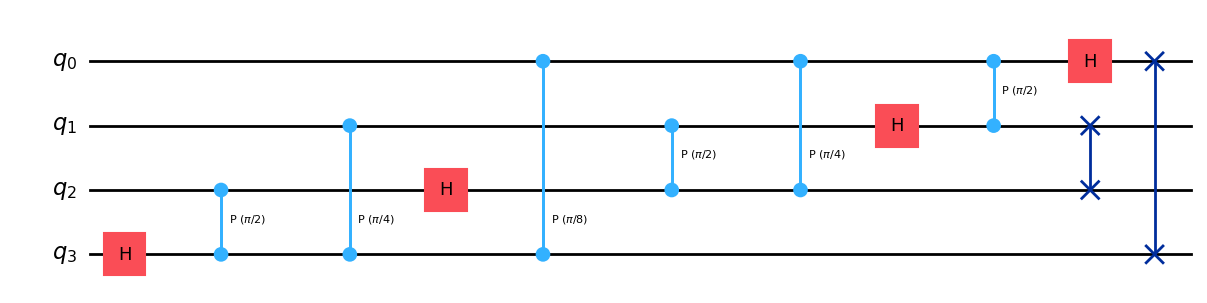
\includegraphics[width=\linewidth]{Images/QFT_2_custom.png}
\end{figure}
Here, we have not used any barriers and thus see a little rearrangements in the gates. This does not affect the computation in any way. Note that because qiskit uses little-endian notation this circuit differs from circuit shown in~\ref{fig:qft_N_withswap}. It could be thought of as mirror image about a horizontal axis. This is because the input $1011$ would be interpreted as $1101$ in qiskit. Thus, to obtain the same manipulations we need to make the circuit in a mirror image about horizontal axis. Same will be followed in the manual implementation of the inverse Fourier transform.

Recall, the matrix for the three qubit Quantum Fourier transform $QFT_3$ using $\omega_8 = e^{2 \pi \iota /8}=\sqrt{i}$, is
\[
QFT_3 = \frac{1}{\sqrt{8}} \begin{pmatrix}
1 & 1 & 1 & 1 & 1 & 1 & 1 & 1 \\
1 & \omega_8 & \omega_8^2 & \omega_8^3 & \omega_8^4 & \omega_8^5 & \omega_8^6 & \omega_8^7 \\
1 & \omega_8^2 & \omega_8^4 & \omega_8^6 & 1 & \omega_8^2 & \omega_8^4 & \omega_8^6 \\
1 & \omega_8^3 & \omega_8^6 & \omega_8 & \omega_8^4 & \omega_8^7 & \omega_8^2 & \omega_8^5 \\
1 & \omega_8^4 & 1 & \omega_8^4 & 1 & \omega_8^4 & 1 & \omega_8^4 \\
1 & \omega_8^5 & \omega_8^2 & \omega_8^7 & \omega_8^4 & \omega_8 & \omega_8^6 & \omega_8^3 \\
1 & \omega_8^6 & \omega_8^4 & \omega_8^2 & 1 & \omega_8^6 & \omega_8^4 & \omega_8^2 \\
1 & \omega_8^7 & \omega_8^6 & \omega_8^5 & \omega_8^4 & \omega_8^3 & \omega_8^2 & \omega_8
\end{pmatrix}
\]
This can also be seen using the following code
\begin{lstlisting}[language=Python]
from qiskit import quantum_info as qi
QFT_matrix = qi.Operator(QFT(n))
print(QFT_matrix.data)
\end{lstlisting}
which outputs the same matrix. Thus, the implemented circuit as well as the qiskit circuit library implementation all are the same.
\subsection{Inverse Quantum Fourier Transform}
The inverse QFT can be obtained by calling the inverse method on this class. The respective code and circuit diagram are:
\begin{lstlisting}[language=Python]
from qiskit import QuantumCircuit
from qiskit.circuit.library import QFT

# Create QFT circuit for 4 qubits
num_qubits = 4
qft_circuit = QFT(num_qubits=num_qubits, approximation_degree=0, do_swaps=True, inverse=False, insert_barriers=True, name="IQFT_2")

# Draw the circuit
qft_circuit.inverse().decompose().draw('mpl')  # Use 'text' if you're in a terminal, 'mpl' if you're in a Jupyter notebook
\end{lstlisting}
\begin{figure}[ht]
    \centering
    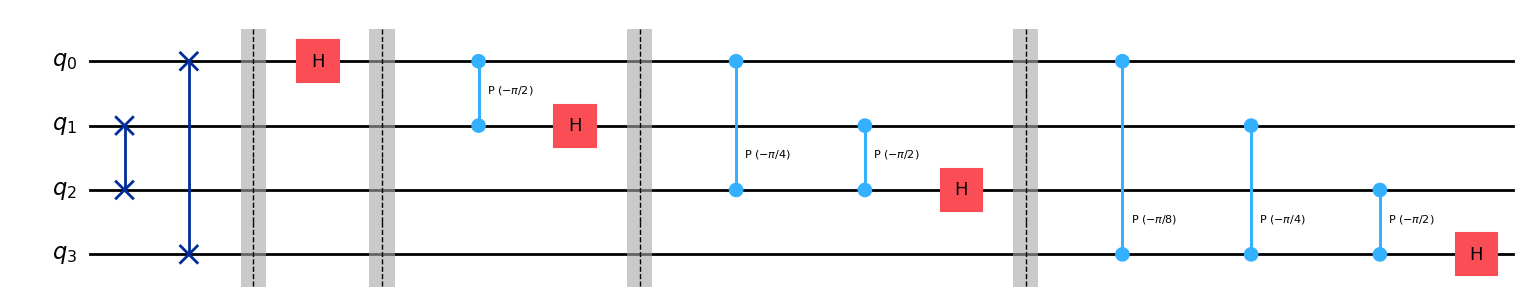
\includegraphics[width=1\linewidth]{Images/IQFT_2.png}
\end{figure}

\begin{table}[ht]
    \centering
    \begin{tabular}{|c|c|}
    \hline
        Circuit name &IQFT\_4\\
        \hline
        Width & 4\\
        \hline
        Depth & 8\\
        \hline
        Total Gates & 12\\
        \hline
        Non-local Gates & 8\\
        \hline
    \end{tabular}
\end{table}
 Note that because Qiskit follows Little Endian notation, the qubits are reversed. So the qubit 0 is the last one on the list. Thus, we have shown how to implement inverse QFT using inbuilt Qiskit circuit library. Now, we will do the same by writing a function for building the Inverse (IQFT) for n qubit. We will now show a manual implementation of the circuit. 
\begin{lstlisting}[language=Python]
def IQFT_custom(n):
    qc_IQFT_custom = QuantumCircuit(n, name='IQFT_2_custom')
    for i in range(n//2):
        qc_IQFT_custom.swap(i,n-i-1)

    for i in range(n):
        qc_IQFT_custom.h(i)
        for j in range(i+1,n):
            qc_IQFT_custom.cp(-np.pi/2**(j-i),j,i)
            
    return qc_IQFT_custom

qc_IQFT_custom = IQFT_custom(4)
qc_IQFT_custom.draw('mpl', filename='../Images/iqft_4_custom.png)
\end{lstlisting}
\begin{figure}[ht]
    \centering
    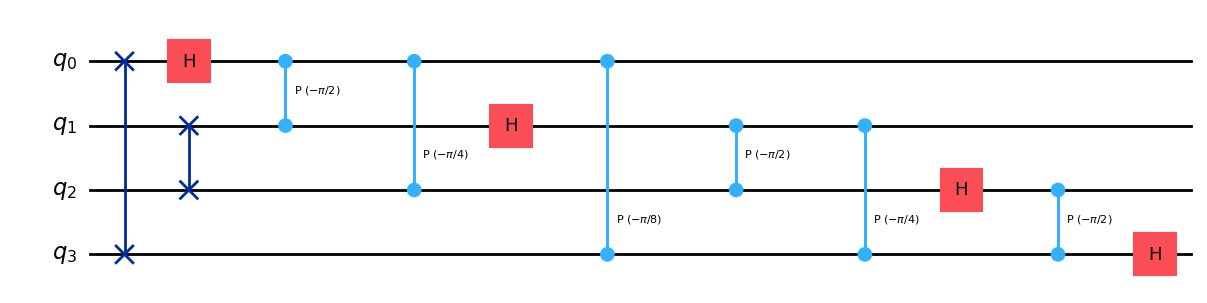
\includegraphics[width=1\linewidth]{Images/IQFT_2_custom.png}
\end{figure}
\subsection{Approximate Quantum Fourier Transform}
Recall that one method to reduce circuit depth is to implement the QFT approximately by ignoring controlled-phase rotations where the angle is beneath a threshold. Here, this can be adjusted using the approximation\_degree attribute: the smallest approximation\_degree rotation angles are dropped from the QFT. For instance, a QFT on 5 qubits with approximation degree 2 yields (the barriers are dropped in this example):
\begin{lstlisting}[language=Python]
qft_circuit = QFT(num_qubits=5, approximation_degree=2, do_swaps=True, inverse=False, insert_barriers=False, name="AQFT_5")

# Draw the circuit
qft_circuit.decompose().draw('mpl')  # Use 'text' if you're in a terminal, 'mpl' if you're in a Jupyter notebook
\end{lstlisting}
\begin{figure}[ht]
    \centering
    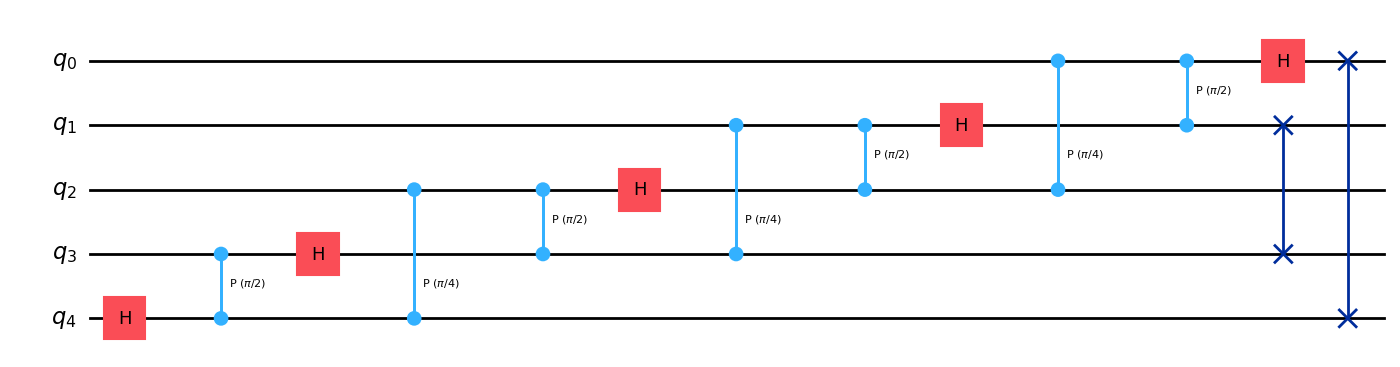
\includegraphics[width=1\linewidth]{Images/AQFT_circ.png}
\end{figure}

\begin{table}[ht]
    \centering
    \begin{tabular}{|c|c|}
    \hline
        Circuit Name & AQFT\_5\\
        \hline
        Width & 5 \\
        \hline
        Depth & 10\\
        \hline
        Total Gates & 14\\
        \hline
        Non-local Gates & 9\\
        \hline
    \end{tabular}
\end{table}
\section{Conclusion}
The best classical algorithms for computing the discrete Fourier transform on $2^n$ elements are algorithms such as the \textit{Fast Fourier Transform (FFT)}, which compute the discrete Fourier transform using $\Theta(n2^n)$ gates/operations. That is, it requires exponentially more operations to compute the Fourier transform on a classical computer than it does to implement the quantum Fourier transform on a quantum computer. At face value, this sounds terrific, since the Fourier transform is a crucial step in so many real-world data processing applications. For example, in computer speech recognition, the first step in phoneme recognition is to Fourier transform the digitized sound. Can we use the quantum Fourier transform to speed up the computations of these Fourier transform? Unfortunately, the answer is that there is no known way to do this. Th problem is that the amplitudes in a quantum computer cannot be directly accessed by measurement. Thus, there is no way of determining the Fourier transformed amplitudes in the original state. Worse still, there is in general no way to efficiently prepare the original state to be Fourier transformed. Thus, finding the uses for the quantum Fourier transform is more subtle than we might have hoped. In the coming chapters we will see several algorithms based upon a more subtle applications of the quantum Fourier transform.










\chapterreferences
